\documentclass[../psets.tex]{subfiles}

\pagestyle{main}
\renewcommand{\leftmark}{Problem Set \thesection}
\setcounter{section}{2}
\setenumerate[2]{label={\alph*)}}

\begin{document}




\section{PCR, Sequencing, Cell Structure, and Localization}
\begin{enumerate}
    \item \marginnote{11/29:}PCR.
    \begin{enumerate}
        \item Can you describe a way to amplify a strand of RNA (i.e., make a large number of [DNA or RNA] copies so that you can submit it for sequencing, for example)? But your challenge is to achieve this using any enzyme (or set of enzymes) except a DNA polymerase. (4 pts)
        \begin{proof}[Answer]
            Given 50-100 copies of the RNA starting material, mix in RNA replicase, NTPs, and 20-30 bp primers. Stick the system into a thermal cycler, allowing repeated annealing, extension, and denaturation steps to take place until the desired quantity of RNA has been synthesized.
        \end{proof}
        \item Professor Tang has invented a new DNA polymerase that produces 3 DNA strands every time it copies a template strand. After 10 cycles of PCR, on a target segment she amplified, how many target DNA strands will she have in the mixture? How many variable length strands will she have in the mixture? 2 bonus points for a mathematical rationale. ($4+2$ pts)
        \begin{proof}[Answer]
            To answer this question, we must make several assumptions:
            \begin{enumerate}
                \item Before the first cycle, there exists a single segment of dsDNA containing the target region as well as some additional base pairs on the sides. It looks like this:
                \begin{figure}[h!]
                    \centering
                    \begin{tikzpicture}
                        \foreach \x in {-2.9,-2.7,...,2.9} {
                            \draw [brx,very thick] (\x,-0.1) -- ++(0,0.2);
                        }
                        \draw [rex,ultra thick]
                            (-3,0.1)  -- ++(2,0) ++(2,0) -- ++(2,0)
                            (-3,-0.1) -- ++(2,0) ++(2,0) -- ++(2,0)
                        ;
                        \draw [grx,ultra thick]
                            (-1,0.1)  -- ++(2,0)
                            (-1,-0.1) -- ++(2,0)
                        ;
                    \end{tikzpicture}
                    \caption{Initial DNA segment.}
                    \label{fig:DNAinit}
                \end{figure}
                \item Every cycle has three steps.
                \begin{figure}[H]
                    \centering
                    \begin{subfigure}[b]{0.4\linewidth}
                        \centering
                        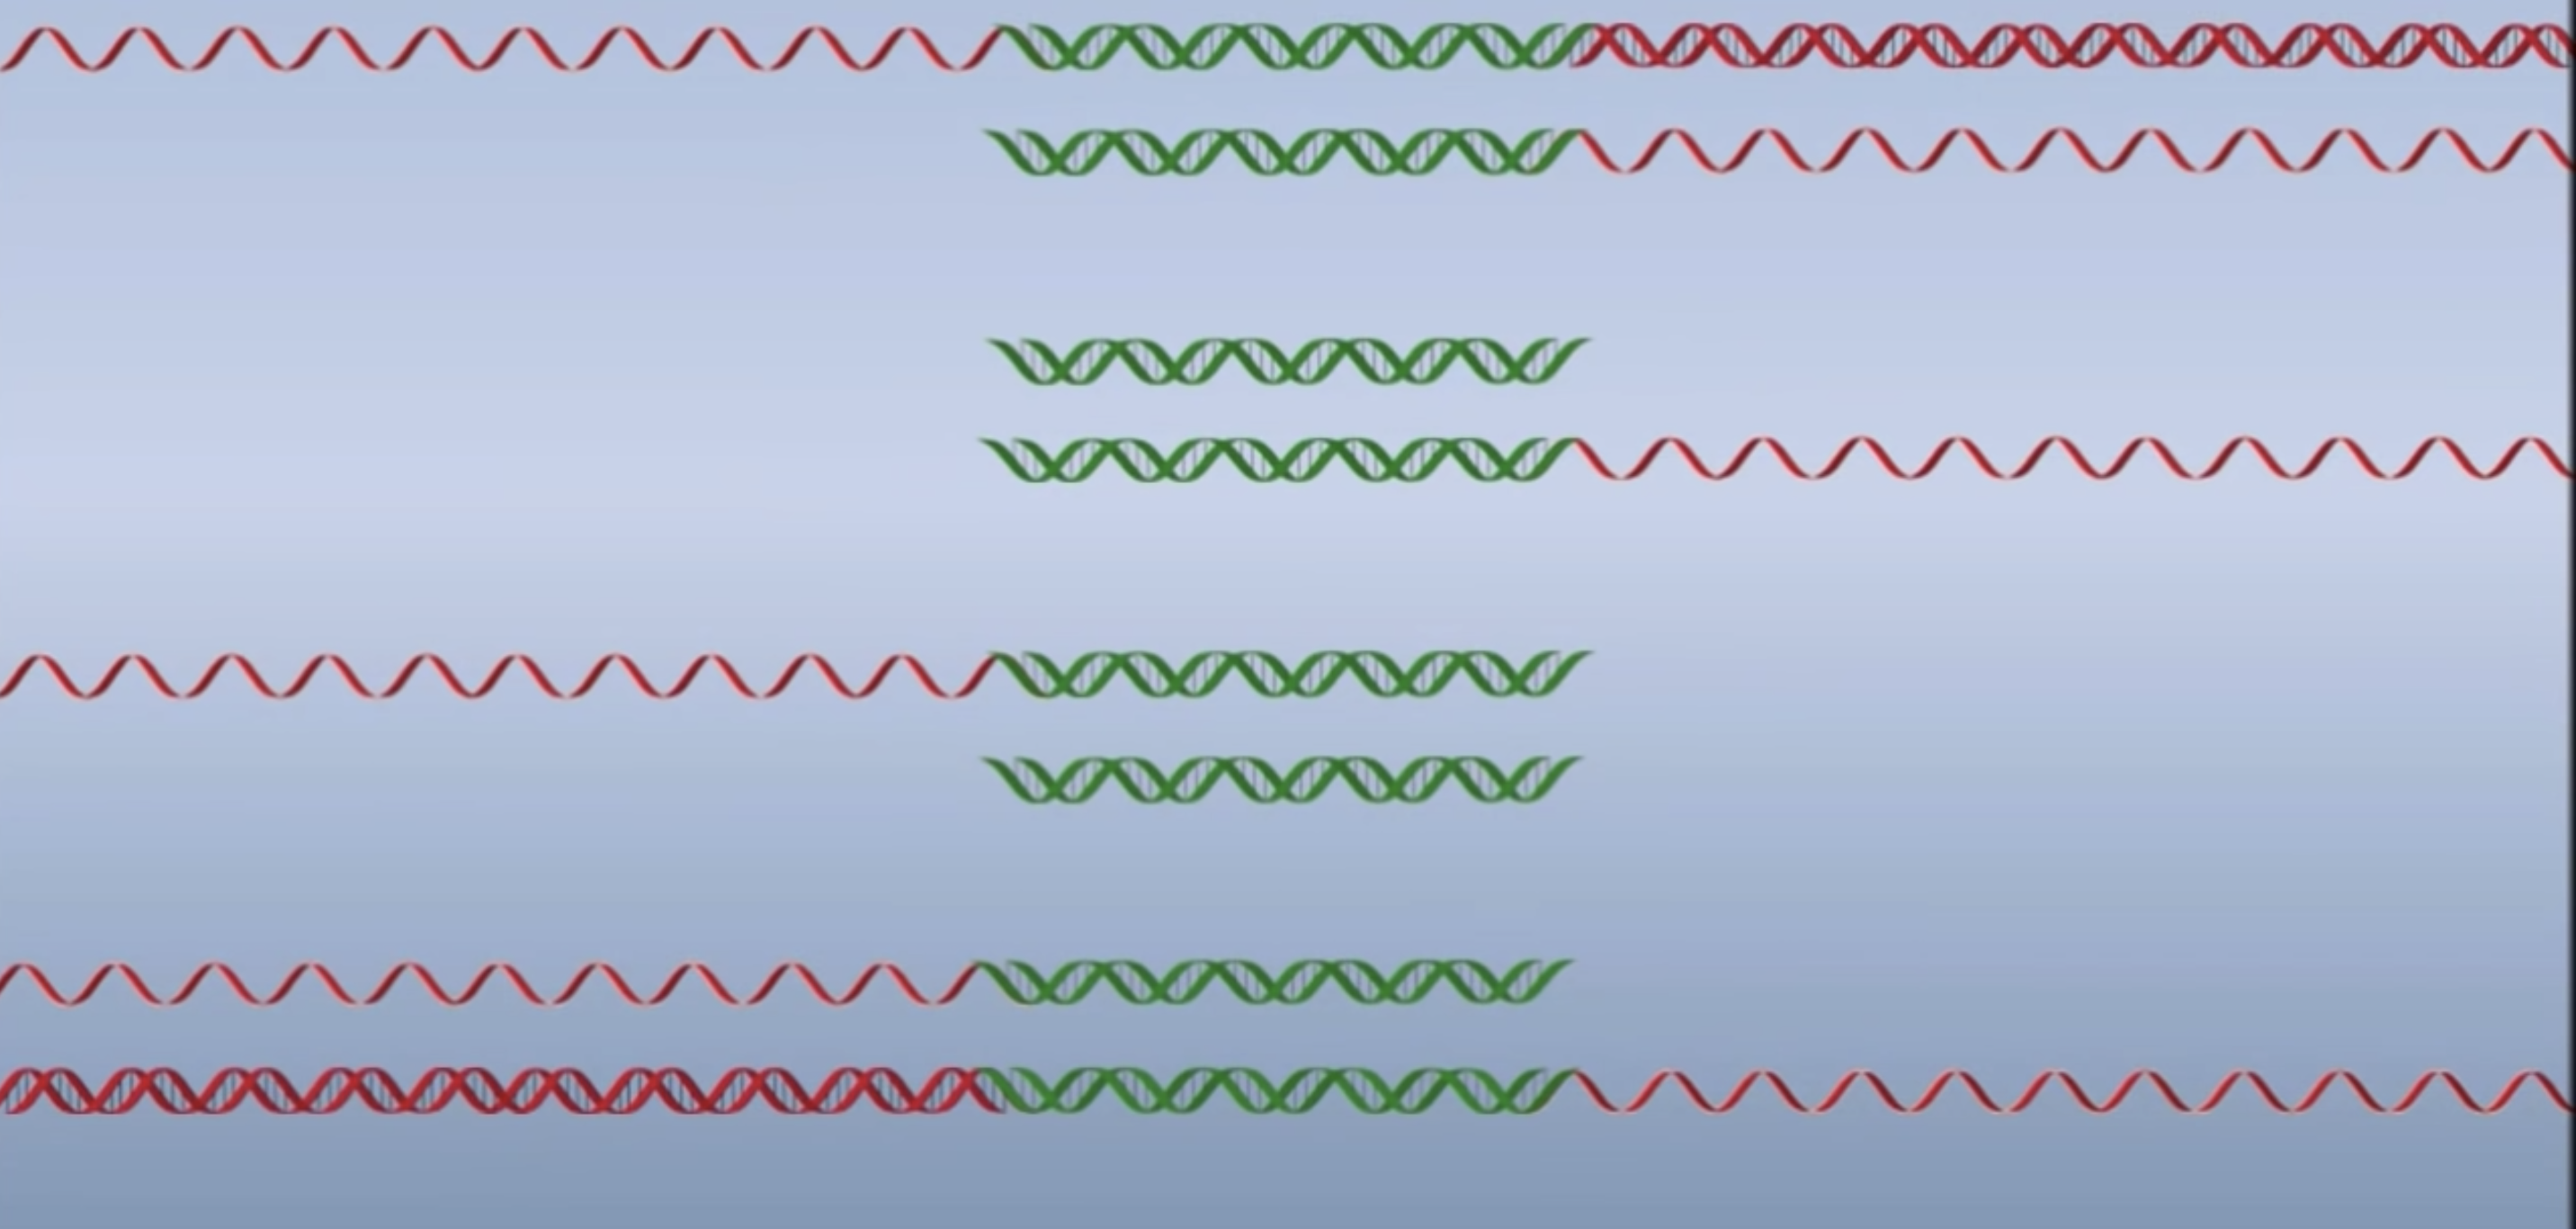
\includegraphics[width=0.9\linewidth]{../ExtFiles/pset3-targetDNAa.png}
                        \caption{DNA after cycle 3.}
                        \label{fig:pset3-targetDNAa}
                    \end{subfigure}
                    \begin{subfigure}[b]{0.4\linewidth}
                        \centering
                        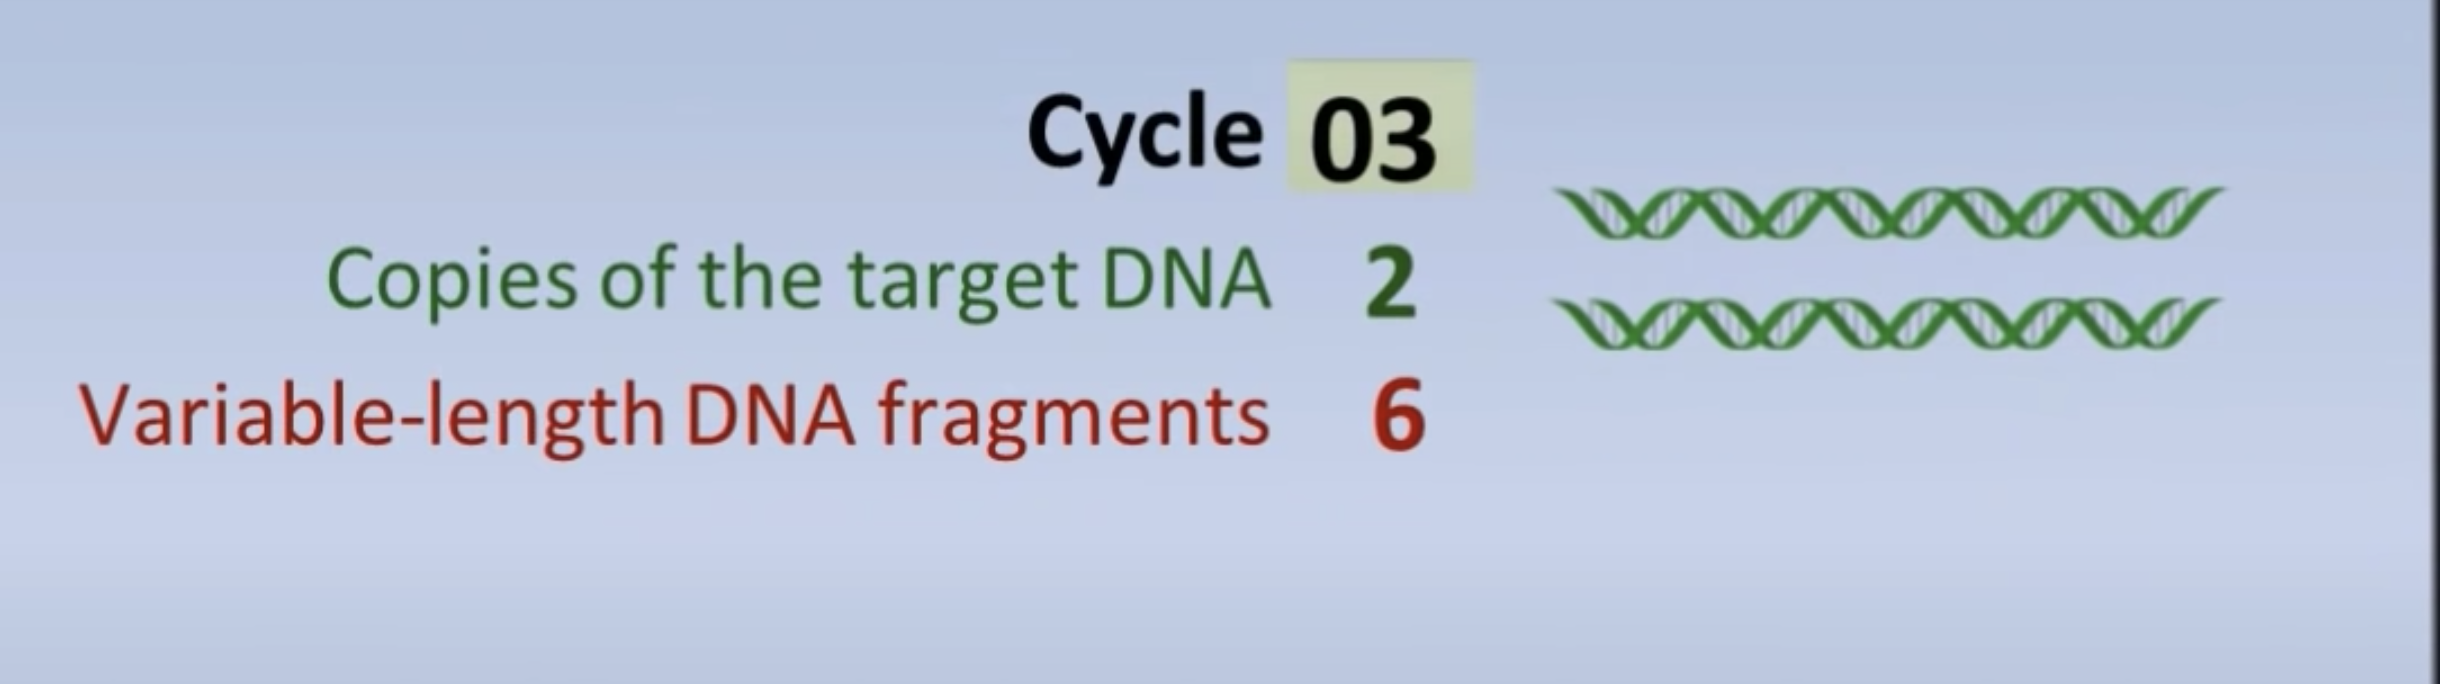
\includegraphics[width=0.9\linewidth]{../ExtFiles/pset3-targetDNAb.png}
                        \caption{Counting DNA after cycle 3.}
                        \label{fig:pset3-targetDNAb}
                    \end{subfigure}
                    \caption{What qualifies as a "target DNA strand?"}
                    \label{fig:targetDNA}
                \end{figure}
                They are denaturation, then annealing, then extension. We count the number of target DNA strands and variable length strands \emph{after} the extension step and \emph{before} the next denaturation step. Thus, two target dsDNA strands (four target ssDNA strands) count as TWO "target DNA strands." All of the composite dsDNA/ssDNA strands count as variable length strands. This convention is taken directly from the video used in class (see Figure \ref{fig:targetDNA}).
                \item On the action of the new DNA polymerase.
                \begin{figure}[H]
                    \centering
                    \begin{tikzpicture}
                        \footnotesize
                        \begin{scope}
                            \foreach \x in {-0.7,-0.6,...,0.7} {
                                \draw [brx,very thick] (\x,-0.1) -- ++(0,0.2);
                            }
                            \draw [rex,ultra thick]
                                (-0.75,0.1)  -- ++(0.5,0) ++(0.5,0) -- ++(0.5,0)
                                (-0.75,-0.1)  -- ++(0.5,0) ++(0.5,0) -- ++(0.5,0)
                            ;
                            \draw [grx,ultra thick]
                                (-0.25,0.1)  -- ++(0.5,0)
                                (-0.25,-0.1) -- ++(0.5,0)
                            ;
                
                            \node at (0,-1.5) {Start point};
                        \end{scope}
                        \draw [-stealth] (1,0) -- node[above]{Denaturation} ++(2,0);
                        \begin{scope}[xshift=4cm]
                            \foreach \x in {-0.7,-0.6,...,0.7} {
                                \draw [brx,very thick]
                                    (\x,1) -- ++(0,-0.1)
                                    (\x,-1) -- ++(0,0.1)
                                ;
                            }
                            \draw [rex,ultra thick]
                                (-0.75,1)  -- ++(0.5,0) ++(0.5,0) -- ++(0.5,0)
                                (-0.75,-1)  -- ++(0.5,0) ++(0.5,0) -- ++(0.5,0)
                            ;
                            \draw [grx,ultra thick]
                                (-0.25,1)  -- ++(0.5,0)
                                (-0.25,-1) -- ++(0.5,0)
                            ;
                        \end{scope}
                        \draw [-stealth] (5,0) -- node[above]{Annealing} ++(1.5,0);
                        \begin{scope}[xshift=7.5cm]
                            \foreach \x in {-0.7,-0.6,...,0.7} {
                                \draw [brx,very thick]
                                    (\x,1) -- ++(0,-0.1)
                                    (\x,-1) -- ++(0,0.1)
                                ;
                            }
                            \draw [rex,ultra thick]
                                (-0.75,1)  -- ++(0.5,0) ++(0.5,0) -- ++(0.5,0)
                                (-0.75,-1)  -- ++(0.5,0) ++(0.5,0) -- ++(0.5,0)
                            ;
                            \draw [grx,ultra thick]
                                (-0.25,1)  -- ++(0.5,0)
                                (-0.25,-1) -- ++(0.5,0)
                            ;
                
                            \draw [brx,very thick]
                                (-0.2,0.9) -- ++(0,-0.1)
                                (-0.1,0.9) -- ++(0,-0.1)
                                (0.1,-0.9) -- ++(0,0.1)
                                (0.2,-0.9) -- ++(0,0.1)
                            ;
                            \draw [ylx,ultra thick]
                                (-0.25,0.8) -- ++(0.2,0)
                                (0.25,-0.8) -- ++(-0.2,0)
                            ;
                        \end{scope}
                        \draw [-stealth] (8.5,0) -- node[above]{Extension} ++(1.5,0);
                        \begin{scope}[xshift=11cm]
                            \foreach \x in {-0.7,-0.6,...,0.7} {
                                \draw [brx,very thick]
                                    (\x,1) -- ++(0,-0.1)
                                    (\x,-1) -- ++(0,0.1)
                                ;
                            }
                            \draw [rex,ultra thick]
                                (-0.75,1)  -- ++(0.5,0) ++(0.5,0) -- ++(0.5,0)
                                (-0.75,-1)  -- ++(0.5,0) ++(0.5,0) -- ++(0.5,0)
                            ;
                            \draw [grx,ultra thick]
                                (-0.25,1)  -- ++(0.5,0)
                                (-0.25,-1) -- ++(0.5,0)
                            ;
                
                            \draw [brx,very thick]
                                (-0.2,0.9) -- ++(0,-0.1)
                                (-0.1,0.9) -- ++(0,-0.1)
                                (0.1,-0.9) -- ++(0,0.1)
                                (0.2,-0.9) -- ++(0,0.1)
                            ;
                            \draw [ylx,ultra thick]
                                (-0.25,0.8) -- ++(0.2,0)
                                (0.25,-0.8) -- ++(-0.2,0)
                            ;
                
                            \draw [brx,very thick]
                                foreach \x in {0,0.1,...,0.75} {
                                    (\x,0.8) -- ++(0,0.1)
                                }
                                foreach \x in {-0.7,-0.6,...,0} {
                                    (\x,-0.9) -- ++(0,0.1)
                                }
                            ;
                            \draw [grx,ultra thick]
                                (-0.05,0.8) -- ++(0.3,0)
                                (0.05,-0.8) -- ++(-0.3,0)
                            ;
                            \draw [rex,ultra thick]
                                (0.25,0.8) -- ++(0.5,0)
                                (-0.25,-0.8) -- ++(-0.5,0)
                            ;
                
                            % 
                
                            \draw [brx,very thick]
                                (-0.2,0.6) -- ++(0,-0.1)
                                (-0.1,0.6) -- ++(0,-0.1)
                                (0.1,-0.6) -- ++(0,0.1)
                                (0.2,-0.6) -- ++(0,0.1)
                            ;
                            \draw [ylx,ultra thick]
                                (-0.25,0.5) -- ++(0.2,0)
                                (0.25,-0.5) -- ++(-0.2,0)
                            ;
                
                            \draw [brx,very thick]
                                foreach \x in {0,0.1,...,0.75} {
                                    (\x,0.5) -- ++(0,0.1)
                                }
                                foreach \x in {-0.7,-0.6,...,0} {
                                    (\x,-0.6) -- ++(0,0.1)
                                }
                            ;
                            \draw [grx,ultra thick]
                                (-0.05,0.5) -- ++(0.3,0)
                                (0.05,-0.5) -- ++(-0.3,0)
                            ;
                            \draw [rex,ultra thick]
                                (0.25,0.5) -- ++(0.5,0)
                                (-0.25,-0.5) -- ++(-0.5,0)
                            ;
                
                            % 
                
                            \draw [brx,very thick]
                                (-0.2,0.3) -- ++(0,-0.1)
                                (-0.1,0.3) -- ++(0,-0.1)
                                (0.1,-0.3) -- ++(0,0.1)
                                (0.2,-0.3) -- ++(0,0.1)
                            ;
                            \draw [ylx,ultra thick]
                                (-0.25,0.2) -- ++(0.2,0)
                                (0.25,-0.2) -- ++(-0.2,0)
                            ;
                
                            \draw [brx,very thick]
                                foreach \x in {0,0.1,...,0.75} {
                                    (\x,0.2) -- ++(0,0.1)
                                }
                                foreach \x in {-0.7,-0.6,...,0} {
                                    (\x,-0.3) -- ++(0,0.1)
                                }
                            ;
                            \draw [grx,ultra thick]
                                (-0.05,0.2) -- ++(0.3,0)
                                (0.05,-0.2) -- ++(-0.3,0)
                            ;
                            \draw [rex,ultra thick]
                                (0.25,0.2) -- ++(0.5,0)
                                (-0.25,-0.2) -- ++(-0.5,0)
                            ;
                        \end{scope}
                        \draw [-stealth] (12,0) -- node[above]{Recombination} ++(2,0);
                        \begin{scope}[xshift=15cm]
                            \foreach \x in {-0.7,-0.6,...,0.7} {
                                \draw [brx,very thick]
                                    (\x,1) -- ++(0,-0.1)
                                    (\x,-1) -- ++(0,0.1)
                                ;
                            }
                            \draw [rex,ultra thick]
                                (-0.75,1)  -- ++(0.5,0) ++(0.5,0) -- ++(0.5,0)
                                (-0.75,-1)  -- ++(0.5,0) ++(0.5,0) -- ++(0.5,0)
                            ;
                            \draw [grx,ultra thick]
                                (-0.25,1)  -- ++(0.5,0)
                                (-0.25,-1) -- ++(0.5,0)
                            ;
                
                            \draw [brx,very thick]
                                (-0.2,0.9) -- ++(0,-0.1)
                                (-0.1,0.9) -- ++(0,-0.1)
                                (0.1,-0.9) -- ++(0,0.1)
                                (0.2,-0.9) -- ++(0,0.1)
                            ;
                            \draw [ylx,ultra thick]
                                (-0.25,0.8) -- ++(0.2,0)
                                (0.25,-0.8) -- ++(-0.2,0)
                            ;
                
                            \draw [brx,very thick]
                                foreach \x in {0,0.1,...,0.75} {
                                    (\x,0.8) -- ++(0,0.1)
                                }
                                foreach \x in {-0.7,-0.6,...,0} {
                                    (\x,-0.9) -- ++(0,0.1)
                                }
                            ;
                            \draw [grx,ultra thick]
                                (-0.05,0.8) -- ++(0.3,0)
                                (0.05,-0.8) -- ++(-0.3,0)
                            ;
                            \draw [rex,ultra thick]
                                (0.25,0.8) -- ++(0.5,0)
                                (-0.25,-0.8) -- ++(-0.5,0)
                            ;
                
                            %
                
                            \draw [brx,very thick]
                                foreach \x in {-0.7,-0.6,...,0.2} {
                                    (\x,0.3) -- ++(0,0.1)
                                }
                                foreach \x in {-0.2,-0.1,...,0.7} {
                                    (\x,0.2) -- ++(0,0.1)
                                }
                            ;
                            \draw [ylx,ultra thick]
                                (0.25,0.4) -- ++(-0.2,0)
                                (-0.25,0.2) -- ++(0.2,0)
                            ;
                            \draw [grx,ultra thick]
                                (-0.25,0.4) -- ++(0.3,0)
                                (0.25,0.2) -- ++(-0.3,0)
                            ;
                            \draw [rex,ultra thick]
                                (-0.75,0.4) -- ++(0.5,0)
                                (0.75,0.2) -- ++(-0.5,0)
                            ;
                
                            %
                
                            \draw [brx,very thick]
                                foreach \x in {-0.7,-0.6,...,0.2} {
                                    (\x,-0.3) -- ++(0,0.1)
                                }
                                foreach \x in {-0.2,-0.1,...,0.7} {
                                    (\x,-0.4) -- ++(0,0.1)
                                }
                            ;
                            \draw [ylx,ultra thick]
                                (0.25,-0.2) -- ++(-0.2,0)
                                (-0.25,-0.4) -- ++(0.2,0)
                            ;
                            \draw [grx,ultra thick]
                                (-0.25,-0.2) -- ++(0.3,0)
                                (0.25,-0.4) -- ++(-0.3,0)
                            ;
                            \draw [rex,ultra thick]
                                (-0.75,-0.2) -- ++(0.5,0)
                                (0.75,-0.4) -- ++(-0.5,0)
                            ;
                
                            \node at (0,-1.5) {Final result};
                        \end{scope}
                    \end{tikzpicture}
                    \caption{Counting procedure for the first cycle.}
                    \label{fig:DNAcount}
                \end{figure}
                We assume that whereas a typical DNA polymerase synthesizes one new complementary DNA (cDNA) strand at a time and binds it to the template strand, the new DNA polymerase still does this but also synthesizes an \emph{additional} two identical cDNA strands that it releases into solution. We postulate the existence of a fourth \textbf{recombination} step directly following extension, in which these additional unbound ssDNA strands bond to complementary ones in solution "for thermodynamic reasons" (we make further assumptions concerning what binds to what below). Modifying assumption (ii), we count target DNA and variable length strands \emph{after} this new recombination step and \emph{before} the next denaturation step in the next cycle. For example, we would count four variable length DNA strands after the first cycle (see Figure \ref{fig:DNAcount}).
            \end{enumerate}
            At this point, we are ready to begin the mathematical derivation. First we enumerate the different types of DNA that can be produced according to our model.
            \begin{table}[h!]
                \centering
                \small
                \renewcommand{\arraystretch}{1.2}
                \begin{tabular}{c|c}
                    \textbf{Type} & \textbf{Presentation}\\
                    \hline
                    1 & \tikz{
                        \foreach \x in {-0.7,-0.6,...,0.7} {
                            \draw [brx,very thick] (\x,-0.1) -- ++(0,0.2);
                        }
                        \draw [rex,ultra thick]
                            (-0.75,0.1)  -- ++(0.5,0) ++(0.5,0) -- ++(0.5,0)
                            (-0.75,-0.1)  -- ++(0.5,0) ++(0.5,0) -- ++(0.5,0)
                        ;
                        \draw [grx,ultra thick]
                            (-0.25,0.1)  -- ++(0.5,0)
                            (-0.25,-0.1) -- ++(0.5,0)
                        ;
                    }\\
                    2 & \tikz{
                        \foreach \x in {-0.7,-0.6,...,0.7} {
                            \draw [brx,very thick]
                                (\x,1) -- ++(0,-0.1)
                            ;
                        }
                        \draw [brx,very thick]
                            foreach \x in {-0.2,-0.1,...,0.75} {
                                (\x,0.8) -- ++(0,0.1)
                            }
                        ;
            
                        \draw [rex,ultra thick] (-0.75,1)  -- ++(0.5,0) ++(0.5,0) -- ++(0.5,0);
                        \draw [grx,ultra thick] (-0.25,1)  -- ++(0.5,0);
                        \draw [ylx,ultra thick] (-0.25,0.8) -- ++(0.2,0);
                        \draw [grx,ultra thick] (-0.05,0.8) -- ++(0.3,0);
                        \draw [rex,ultra thick] (0.25,0.8) -- ++(0.5,0);
                    }\\
                    3 & \tikz{
                        \foreach \x in {-0.7,-0.6,...,0.7} {
                            \draw [brx,very thick]
                                (\x,-1) -- ++(0,0.1)
                            ;
                        }
                        \draw [brx,very thick]
                            foreach \x in {-0.7,-0.6,...,0.2} {
                                (\x,-0.9) -- ++(0,0.1)
                            }
                        ;
            
                        \draw [rex,ultra thick] (-0.75,-1)  -- ++(0.5,0) ++(0.5,0) -- ++(0.5,0);
                        \draw [grx,ultra thick] (-0.25,-1) -- ++(0.5,0);
                        \draw [ylx,ultra thick] (0.25,-0.8) -- ++(-0.2,0);
                        \draw [grx,ultra thick] (0.05,-0.8) -- ++(-0.3,0);
                        \draw [rex,ultra thick] (-0.25,-0.8) -- ++(-0.5,0);
                    }\\
                    % 4 & \tikz{
                    %     \draw [brx,very thick]
                    %         foreach \x in {-0.2,-0.1,...,0.75} {
                    %             (\x,0.3) -- ++(0,0.1)
                    %         }
                    %         foreach \x in {-0.7,-0.6,...,0.2} {
                    %             (\x,0.2) -- ++(0,0.1)
                    %         }
                    %     ;
                    %     \draw [ylx,ultra thick]
                    %         (-0.25,0.4) -- ++(0.2,0)
                    %         (0.25,0.2) -- ++(-0.2,0)
                    %     ;
                    %     \draw [grx,ultra thick]
                    %         (-0.05,0.4) -- ++(0.3,0)
                    %         (0.05,0.2) -- ++(-0.3,0)
                    %     ;
                    %     \draw [rex,ultra thick]
                    %         (0.25,0.4) -- ++(0.5,0)
                    %         (-0.25,0.2) -- ++(-0.5,0)
                    %     ;
                    % }\\
                    4 & \tikz{
                        \draw [brx,very thick]
                            foreach \x in {-0.7,-0.6,...,0.2} {
                                (\x,0.3) -- ++(0,0.1)
                            }
                            foreach \x in {-0.2,-0.1,...,0.7} {
                                (\x,0.2) -- ++(0,0.1)
                            }
                        ;
                        \draw [ylx,ultra thick]
                            (0.25,0.4) -- ++(-0.2,0)
                            (-0.25,0.2) -- ++(0.2,0)
                        ;
                        \draw [grx,ultra thick]
                            (0.05,0.4) -- ++(-0.3,0)
                            (-0.05,0.2) -- ++(0.3,0)
                        ;
                        \draw [rex,ultra thick]
                            (-0.75,0.4) -- ++(0.5,0)
                            (0.25,0.2) -- ++(0.5,0)
                        ;
                    }\\
                    5 & \tikz{
                        \foreach \x in {-0.2,-0.1,...,0.2} {
                            \draw [brx,very thick]
                                (\x,1) -- ++(0,-0.1)
                            ;
                        }
                        \draw [brx,very thick]
                            foreach \x in {-0.2,-0.1,...,0.75} {
                                (\x,0.8) -- ++(0,0.1)
                            }
                        ;
            
                        \draw [ylx,ultra thick] (-0.25,0.8) -- ++(0.2,0);
                        \draw [grx,ultra thick] (-0.05,0.8) -- ++(0.3,0);
                        \draw [rex,ultra thick] (0.25,0.8) -- ++(0.5,0);
                        \draw [grx,ultra thick] (-0.25,1)  -- ++(0.3,0);
                        \draw [ylx,ultra thick] (0.05,1) -- ++(0.2,0);
            
                        \path (-0.75,1) -- ++(0.5,0);
                    }\\
                    6 & \tikz{
                        \foreach \x in {-0.2,-0.1,...,0.2} {
                            \draw [brx,very thick]
                                (\x,-1) -- ++(0,0.1)
                            ;
                        }
                        \draw [brx,very thick]
                            foreach \x in {-0.7,-0.6,...,0.2} {
                                (\x,-0.9) -- ++(0,0.1)
                            }
                        ;
            
                        \draw [ylx,ultra thick] (0.25,-0.8) -- ++(-0.2,0);
                        \draw [grx,ultra thick] (0.05,-0.8) -- ++(-0.3,0);
                        \draw [rex,ultra thick] (-0.25,-0.8) -- ++(-0.5,0);
                        \draw [grx,ultra thick] (-0.05,-1) -- ++(0.3,0);
                        \draw [ylx,ultra thick] (-0.25,-1) -- ++(0.2,0);
            
                        \path (0.25,-1) -- ++(0.5,0);
                    }\\
                    7 & \tikz{
                        \draw [brx,very thick]
                            foreach \x in {-0.2,-0.1,...,0.75} {
                                (\x,0.3) -- ++(0,0.1)
                            }
                            foreach \x in {-0.2,-0.1,...,0.2} {
                                (\x,0.2) -- ++(0,0.1)
                            }
                        ;
                        \draw [ylx,ultra thick]
                            (-0.25,0.4) -- ++(0.2,0)
                            (0.25,0.2) -- ++(-0.2,0)
                        ;
                        \draw [grx,ultra thick]
                            (-0.05,0.4) -- ++(0.3,0)
                            (0.05,0.2) -- ++(-0.3,0)
                        ;
                        \draw [rex,ultra thick]
                            (0.25,0.4) -- ++(0.5,0)
                        ;
            
                        \path (-0.75,0.4) -- ++(0.5,0);
                    }\\
                    8 & \tikz{
                        \draw [brx,very thick]
                            foreach \x in {-0.2,-0.1,...,0.2} {
                                (\x,0.3) -- ++(0,0.1)
                            }
                            foreach \x in {-0.7,-0.6,...,0.2} {
                                (\x,0.2) -- ++(0,0.1)
                            }
                        ;
                        \draw [ylx,ultra thick]
                            (-0.25,0.4) -- ++(0.2,0)
                            (0.25,0.2) -- ++(-0.2,0)
                        ;
                        \draw [grx,ultra thick]
                            (-0.05,0.4) -- ++(0.3,0)
                            (0.05,0.2) -- ++(-0.3,0)
                        ;
                        \draw [rex,ultra thick]
                            (-0.25,0.2) -- ++(-0.5,0)
                        ;
            
                        \path (0.25,0.4) -- ++(0.5,0);
                    }\\
                    9 & \tikz{
                        \draw [brx,very thick]
                            foreach \x in {-0.2,-0.1,...,0.2} {
                                (\x,0.3) -- ++(0,0.1)
                            }
                            foreach \x in {-0.2,-0.1,...,0.2} {
                                (\x,0.2) -- ++(0,0.1)
                            }
                        ;
                        \draw [ylx,ultra thick]
                            (-0.25,0.4) -- ++(0.2,0)
                            (0.25,0.2) -- ++(-0.2,0)
                        ;
                        \draw [grx,ultra thick]
                            (-0.05,0.4) -- ++(0.3,0)
                            (0.05,0.2) -- ++(-0.3,0)
                        ;
                    }\\
                \end{tabular}
                \caption{Types of DNA.}
                \label{tab:DNAtypes}
            \end{table}
            Now we investigate what is produced during a cycle when each of the above types is present. Let's begin.\par\smallskip
            \underline{Type 1 DNA:} As we can see in Figure \ref{fig:DNAcount}, a single segment of Type 1 DNA will lead to the generation of one Type 2 segment, one Type 3 segment, and two Type 4 segments. We will not explicitly draw out the counting procedure for the other types as we did in Figure \ref{fig:DNAcount}, but we will do our best to rationalize with words.\par
            \underline{Type 2 DNA:} From the top strand, we get another Type 2 and two single strands for recombination. We will say that each of these single strands joins with an analogous one from Type 3 to form a Type 4. Thus, we say that from the top strand, we get one Type 2 and one Type 4 on average. From the bottom strand, we get a Type 5 and two other single strands for recombination. Again, we will pair these with the analogous ones from Type 3 to form Type 9s. Thus, we say that from the bottom strand, we get one Type 5 and one Type 9.\par
            \underline{Type 3 DNA:} Similarly to Type 2, we get one Type 3, one Type 4, one Type 6, and one Type 9 on average.\par
            \underline{Type 4 DNA:} We get one Type 5, one Type 6, and two Type 9s on average.\par
            \underline{Type 5 DNA:} We get one Type 5 and three Type 9s on average.\par
            \underline{Type 6 DNA:} We get one Type 6 and three Type 9s on average.\par
            \underline{Type 7 DNA:} We get one Type 7 and three Type 9s on average.\par
            \underline{Type 8 DNA:} We get one Type 8 and three Type 9s on average.\par
            \underline{Type 9 DNA:} We get four Type 9s.\par\smallskip
            A natural way to represent all of this data is using matrices. Indeed, the following matrix $M$ summarizes all of the above insights, and acts on the initial condition vector $x_0\in\mathbb{R}^9$ defined by $x_0=(1,0,0,0,0,0,0,0,0)^T$.\par
            \begin{equation*}
                M =
                \begin{pmatrix}
                    0 & 0 & 0 & 0 & 0 & 0 & 0 & 0 & 0\\
                    1 & 1 & 0 & 0 & 0 & 0 & 0 & 0 & 0\\
                    1 & 0 & 1 & 0 & 0 & 0 & 0 & 0 & 0\\
                    2 & 1 & 1 & 0 & 0 & 0 & 0 & 0 & 0\\
                    0 & 1 & 0 & 1 & 1 & 0 & 0 & 0 & 0\\
                    0 & 0 & 1 & 1 & 0 & 1 & 0 & 0 & 0\\
                    0 & 0 & 0 & 0 & 0 & 0 & 1 & 0 & 0\\
                    0 & 0 & 0 & 0 & 0 & 0 & 0 & 1 & 0\\
                    0 & 1 & 1 & 2 & 3 & 3 & 3 & 3 & 4\\
                \end{pmatrix}
            \end{equation*}
            Notice that we have, for example, $Mx_0=(0,1,1,2,0,0,0,0,0,0)^T$, as expected: The physical interpretation of the vector $Mx_0$ is that after cycle 1, we should expect one Type 2 segment, one Type 3 segment, and two Type 4 segments, as depicted in Figure \ref{fig:DNAcount}.\par
            To compute the number of strands of each type after 10 cycles, we compute
            \begin{equation*}
                M^{10}x_0 =
                \begin{pmatrix}
                    0\\
                    1\\
                    1\\
                    2\\
                    27\\
                    27\\
                    0\\
                    0\\
                    \num{1048518}\\
                \end{pmatrix}
            \end{equation*}
            The bottommost number in the above vector corresponds to the number of Type 10 DNA segments (target DNA strands) after 10 cycles. The rest of the numbers correspond to variable length strands of the various types; their sum is the total number of variable length strands in the mixture. Therefore, there are approximately
            \begin{equation*}
                \boxed{\num{1048518}\text{ target DNA strands}}
            \end{equation*}
            and
            \begin{equation*}
                \boxed{58\text{ variable length strands}}
            \end{equation*}
            in the mixture.\par
            Note that as per the 11/29 Canvas announcement on this subject, it appears that we may want to count the pairs of \emph{all} target DNA strands produced, including those I counted as bound up in Types 5, 6, 7, and 8 DNA segments at the conclusion of the 10 cycles. If this is the proper assumption, then since there are $27+27+0+0=54$ variable length strands of these types (containing 54 ssDNA strands which pair to $54/2=27$ additional target DNA strands and 27 fewer variable length strands) we adjust our counts to
            \begin{align*}
                \num{1048518}+27 &= \num{1048545}&
                58-27 &= 31
            \end{align*}
            An alternate way to get this latter answer would be to make the following two observations. First, notice that the \emph{total} number of strands is $4^n$ following $n$ cycles. Second, notice that the only ssDNA strands that can produce new variable length ssDNA are the original two. Together, these account for the production of six new non-target (hence variable) ssDNA strands per cycle, or three new variable length dsDNA strands per cycle. Thus, the number of variable length strands is $1+3n$ following $n$-cycles. It follows that after 10 cycles, we would have $4^{10}=\num{1048576}$ total strands and $1+3(10)=31$ variable length strands. Therefore, since $\text{target}=\text{total}-\text{variable}$, we have
            \begin{align*}
                \num{1048576}-31 &= \num{1048545}&
                31 &
            \end{align*} 
            target DNA and variable length strands, respectively, in agreement with the above.
        \end{proof}
    \end{enumerate}
    \item Sequencing.\par
    In Maxam-Gilbert sequencing, the 4 nucleotides A, T, G, and C react in 4 specific reactions, leading to the strand being cleaved when it is treated with hot piperidine. For each nucleobase, write below the chemical reaction that occurs, and how the strand gets cleaved. Hefty bonus points for the reaction mechanism. ($4\times 1$ pt for the reaction; $4\times 2$ pts for the reaction mechanism)
    \begin{proof}[Answer]
        Each strand gets cleaved \emph{at} the targeted nucleotide; in other words, the reagents we use heavily disfigure the targeted nucleotide and eventually cleave it from both the $5'$ and $3'$ sides. In Maxam-Gilbert sequencing, the $5'$ side, minus the modified/disfigured nucleotide and the rest of the chain that follows it to the $3'$ end, will go on to show up in the final radiograph.\par
        Below are the net reactions --- and mechanisms --- for the reaction of guanine with \ce{Me2SO4} followed by hot piperidine, adenine and formic acid followed by hot piperidine (there is also a guanine variant that will not be shown), cytosine and hydrazine/sodium chloride followed by hot piperidine, and thymine and hydrazine followed by hot piperidine (there is also a cytosine variant that will not be shown). All reactions occur in aqueous (often basic) media. Some parts of later reaction mechanisms are left off because of complete homology to preceding mechanisms; a note is always made when this is the case.\par
        Without further ado, here are the results.
        \begin{figure}[H]
            \centering
            \begin{subfigure}[b]{\linewidth}
                \centering
                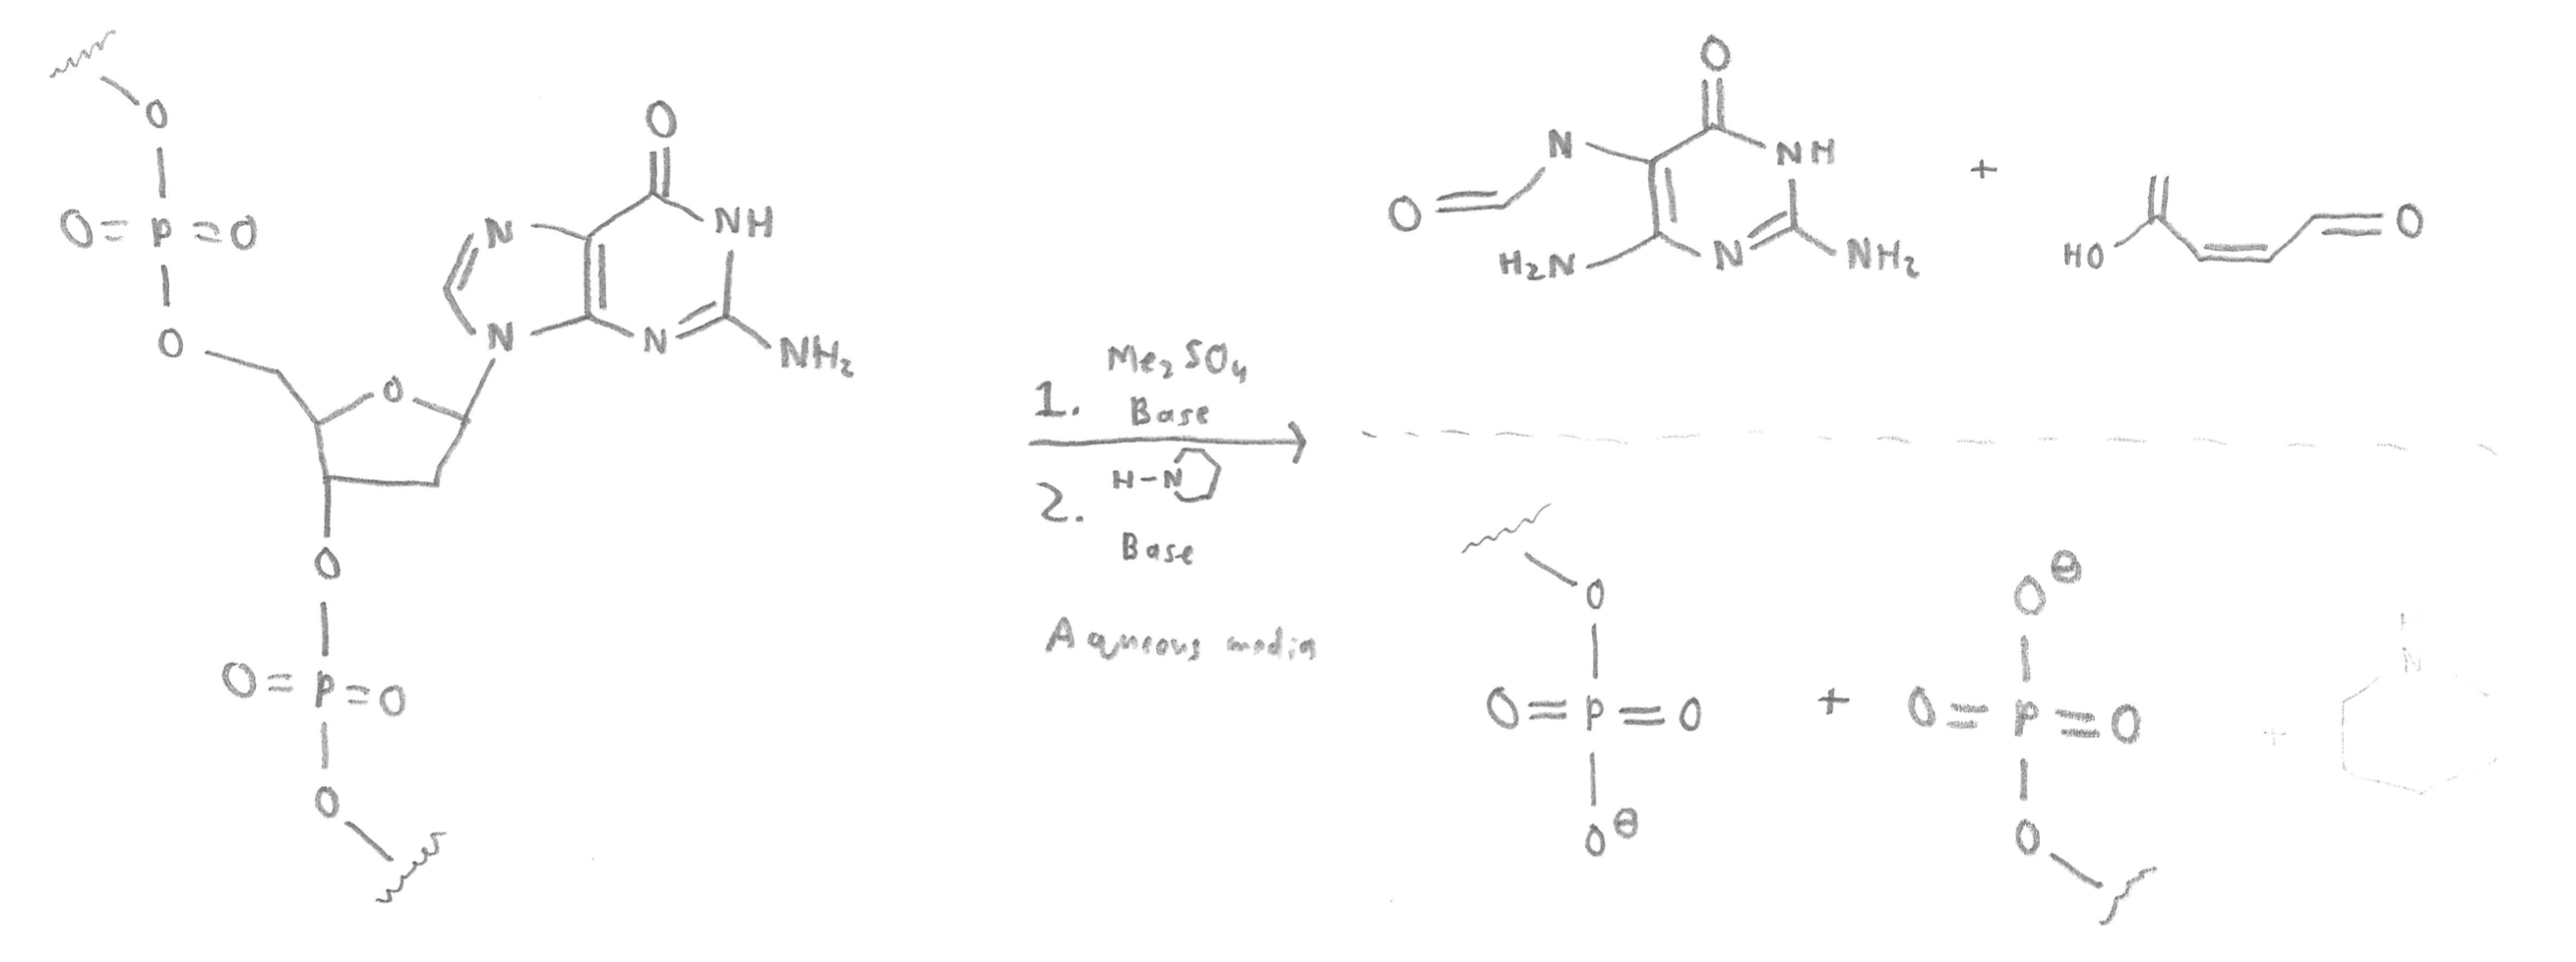
\includegraphics[width=\linewidth]{../ExtFiles/pset3-netRxnG.png}
                \caption{G.}
                \label{fig:pset3-netRxnG}
            \end{subfigure}\\[2em]
            \begin{subfigure}[b]{\linewidth}
                \centering
                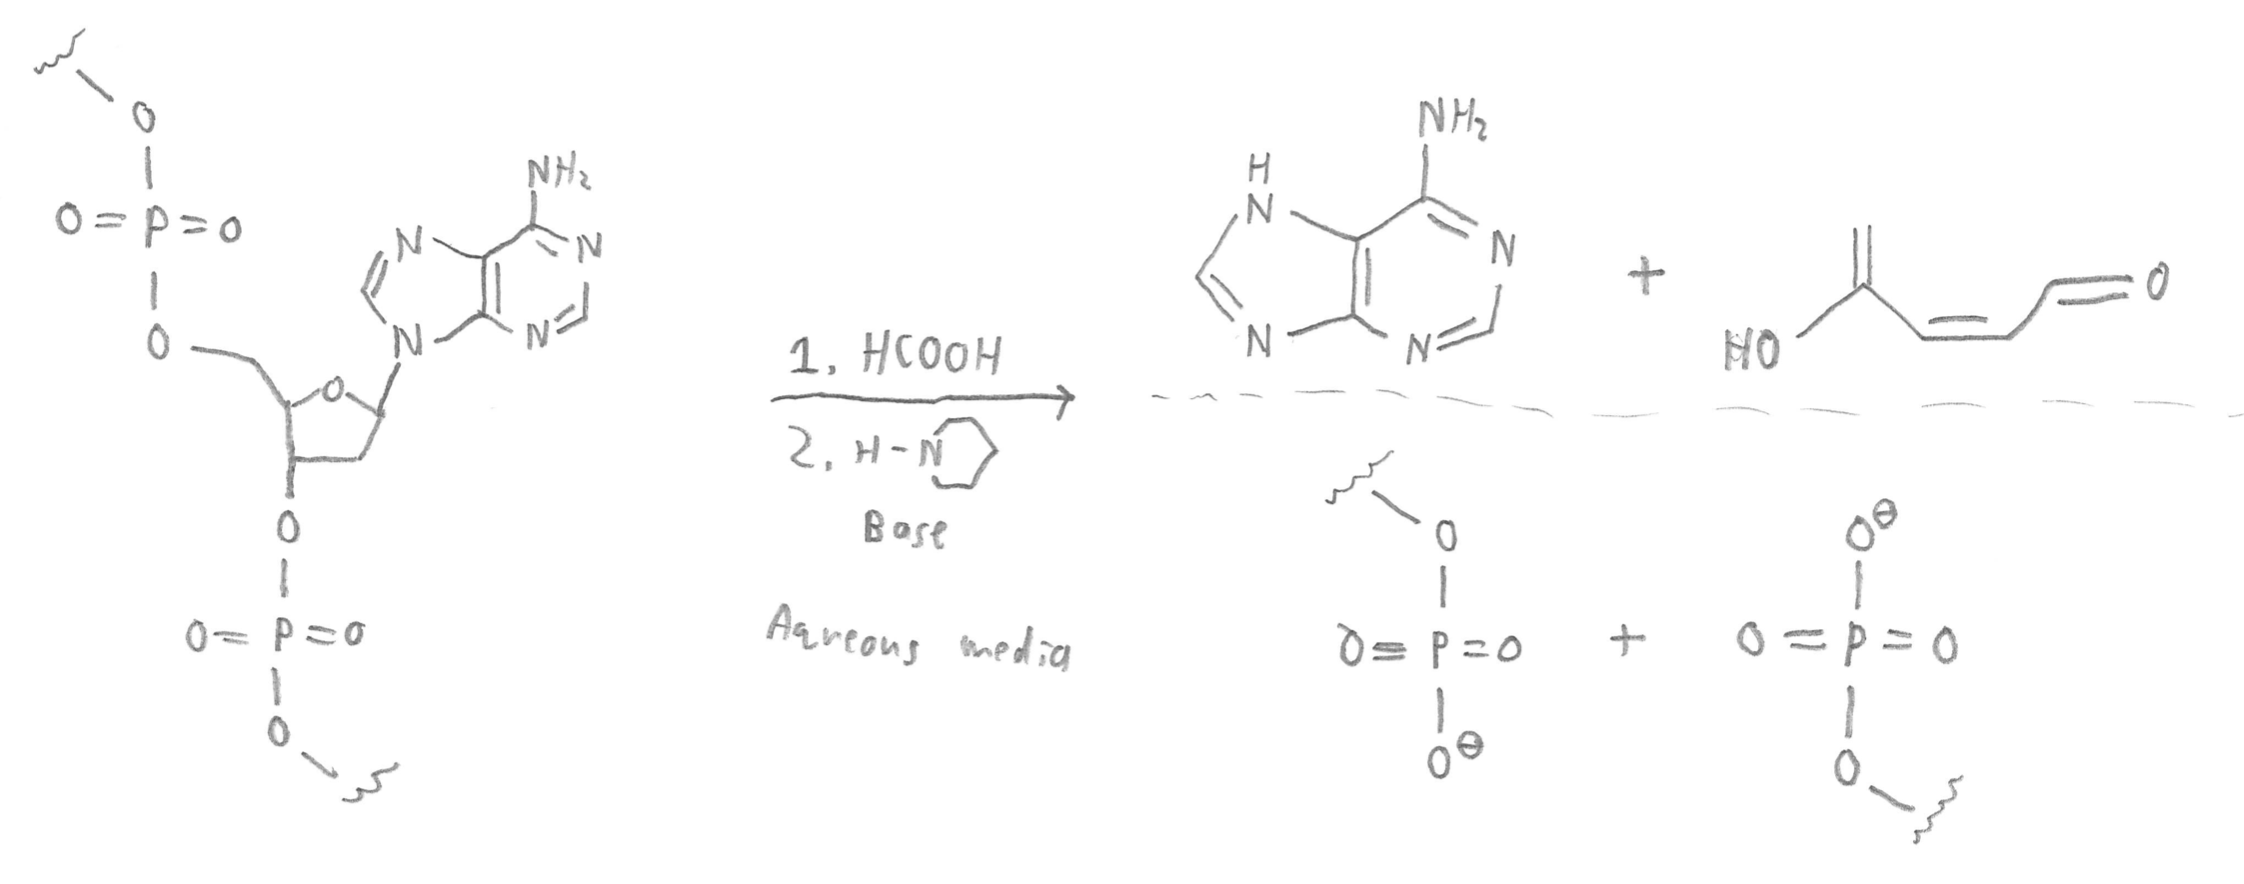
\includegraphics[width=\linewidth]{../ExtFiles/pset3-netRxnA.png}
                \caption{A.}
                \label{fig:pset3-netRxnA}
            \end{subfigure}
        \end{figure}
        \begin{figure}[H]
            \ContinuedFloat
            \centering
            \begin{subfigure}[b]{\linewidth}
                \centering
                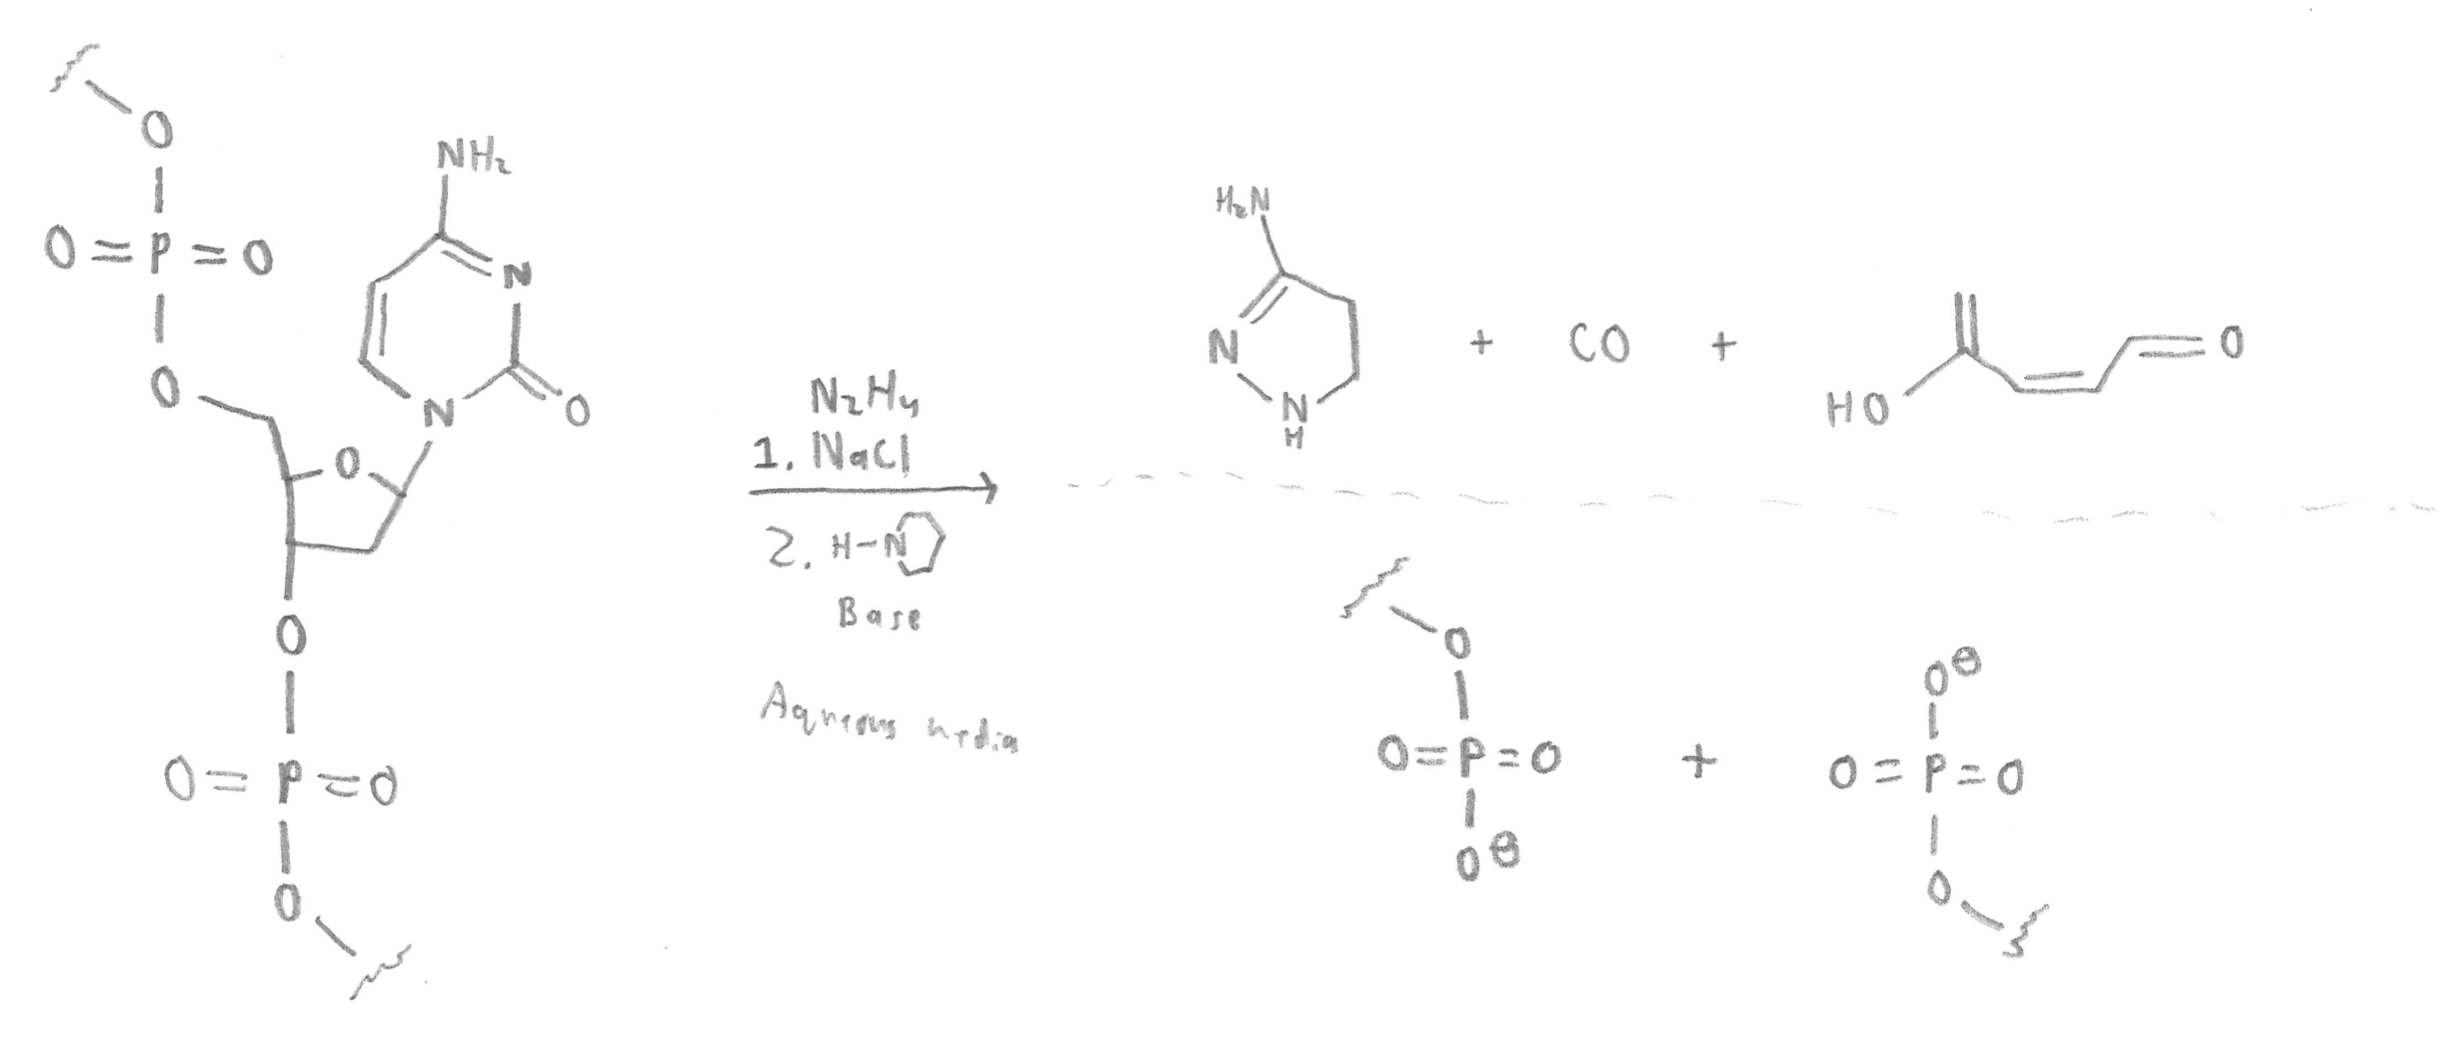
\includegraphics[width=\linewidth]{../ExtFiles/pset3-netRxnC.png}
                \caption{C.}
                \label{fig:pset3-netRxnC}
            \end{subfigure}\\[2em]
            \begin{subfigure}[b]{\linewidth}
                \centering
                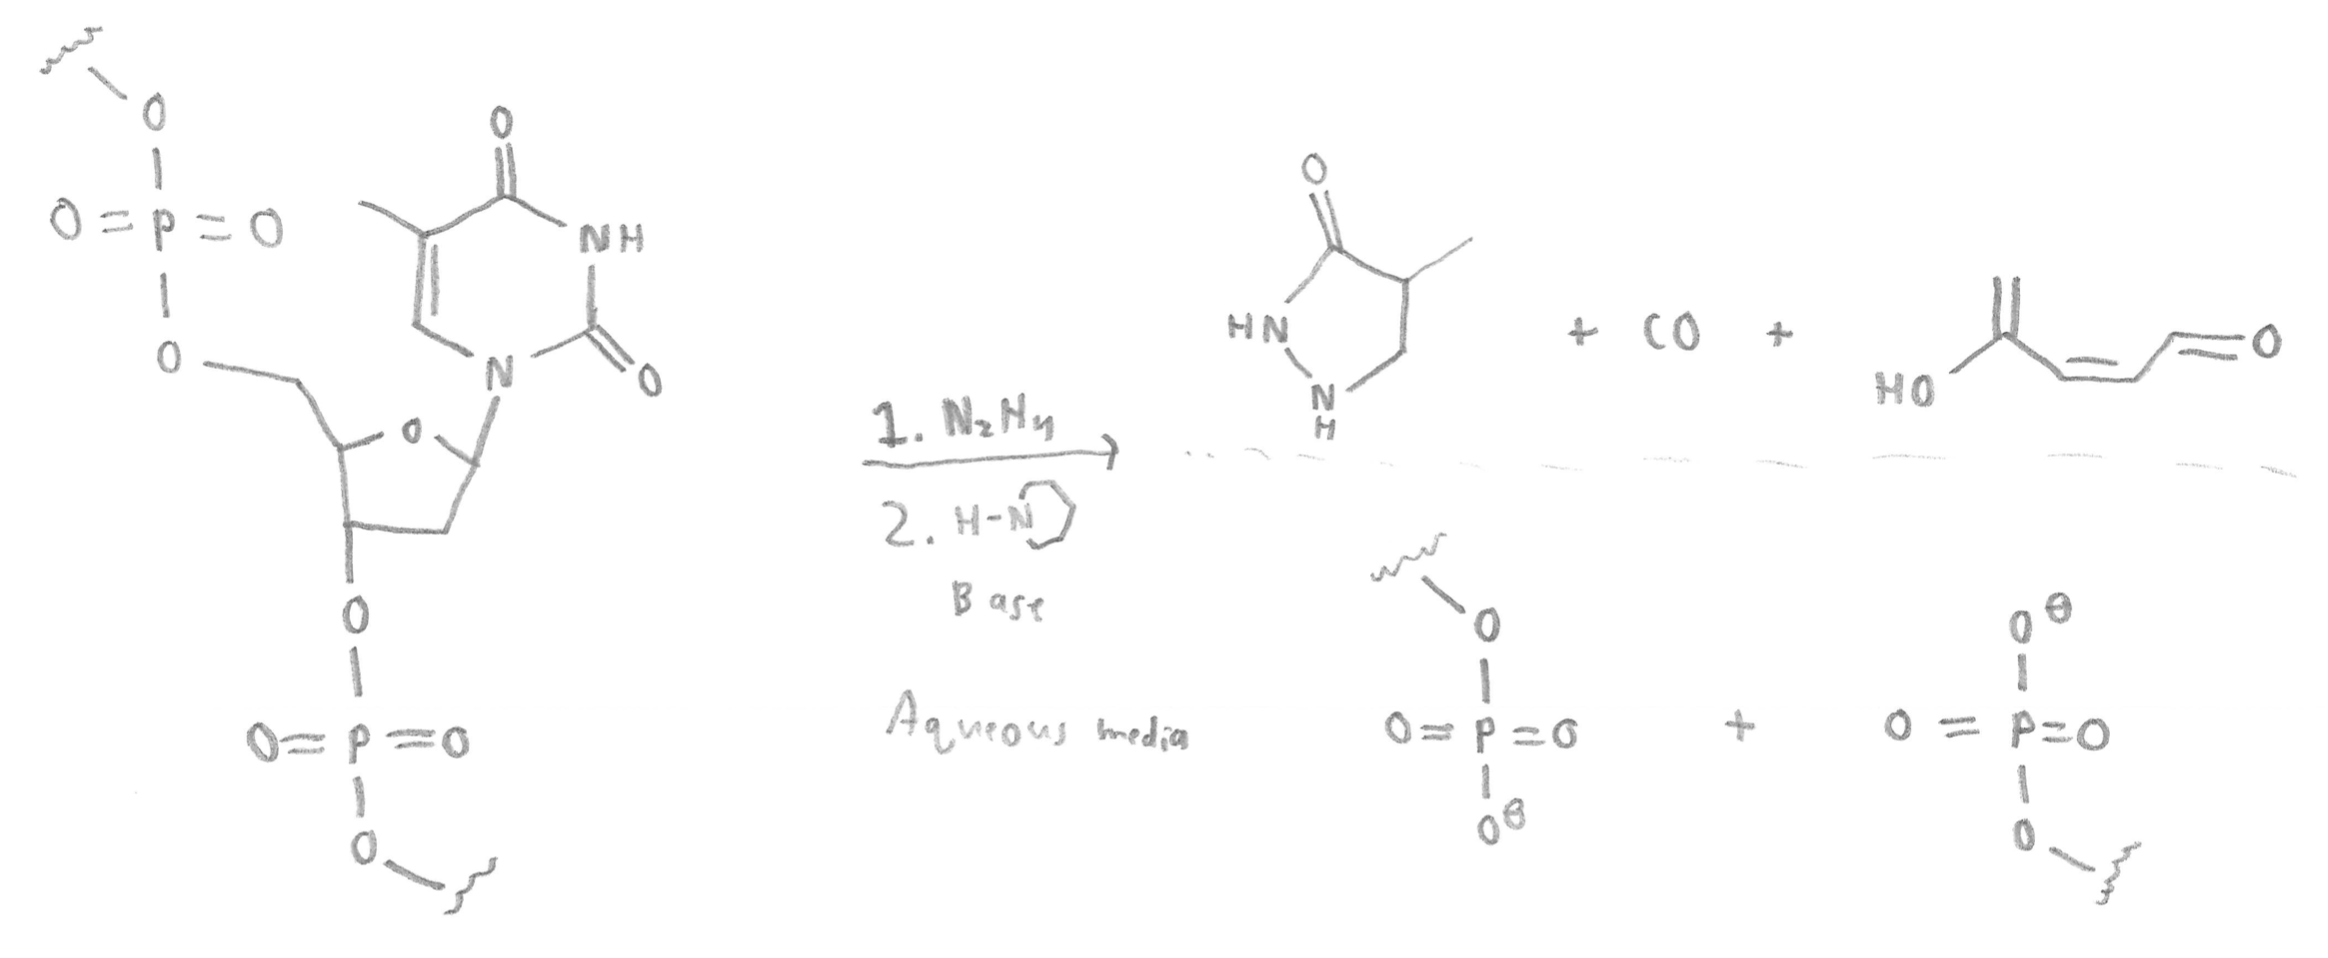
\includegraphics[width=\linewidth]{../ExtFiles/pset3-netRxnT.png}
                \caption{T.}
                \label{fig:pset3-netRxnT}
            \end{subfigure}
            \caption{Net reactions.}
            \label{fig:pset3-netRxn}
        \end{figure}
        \begin{figure}[H]
            \centering
            \begin{subfigure}[b]{\linewidth}
                \centering
                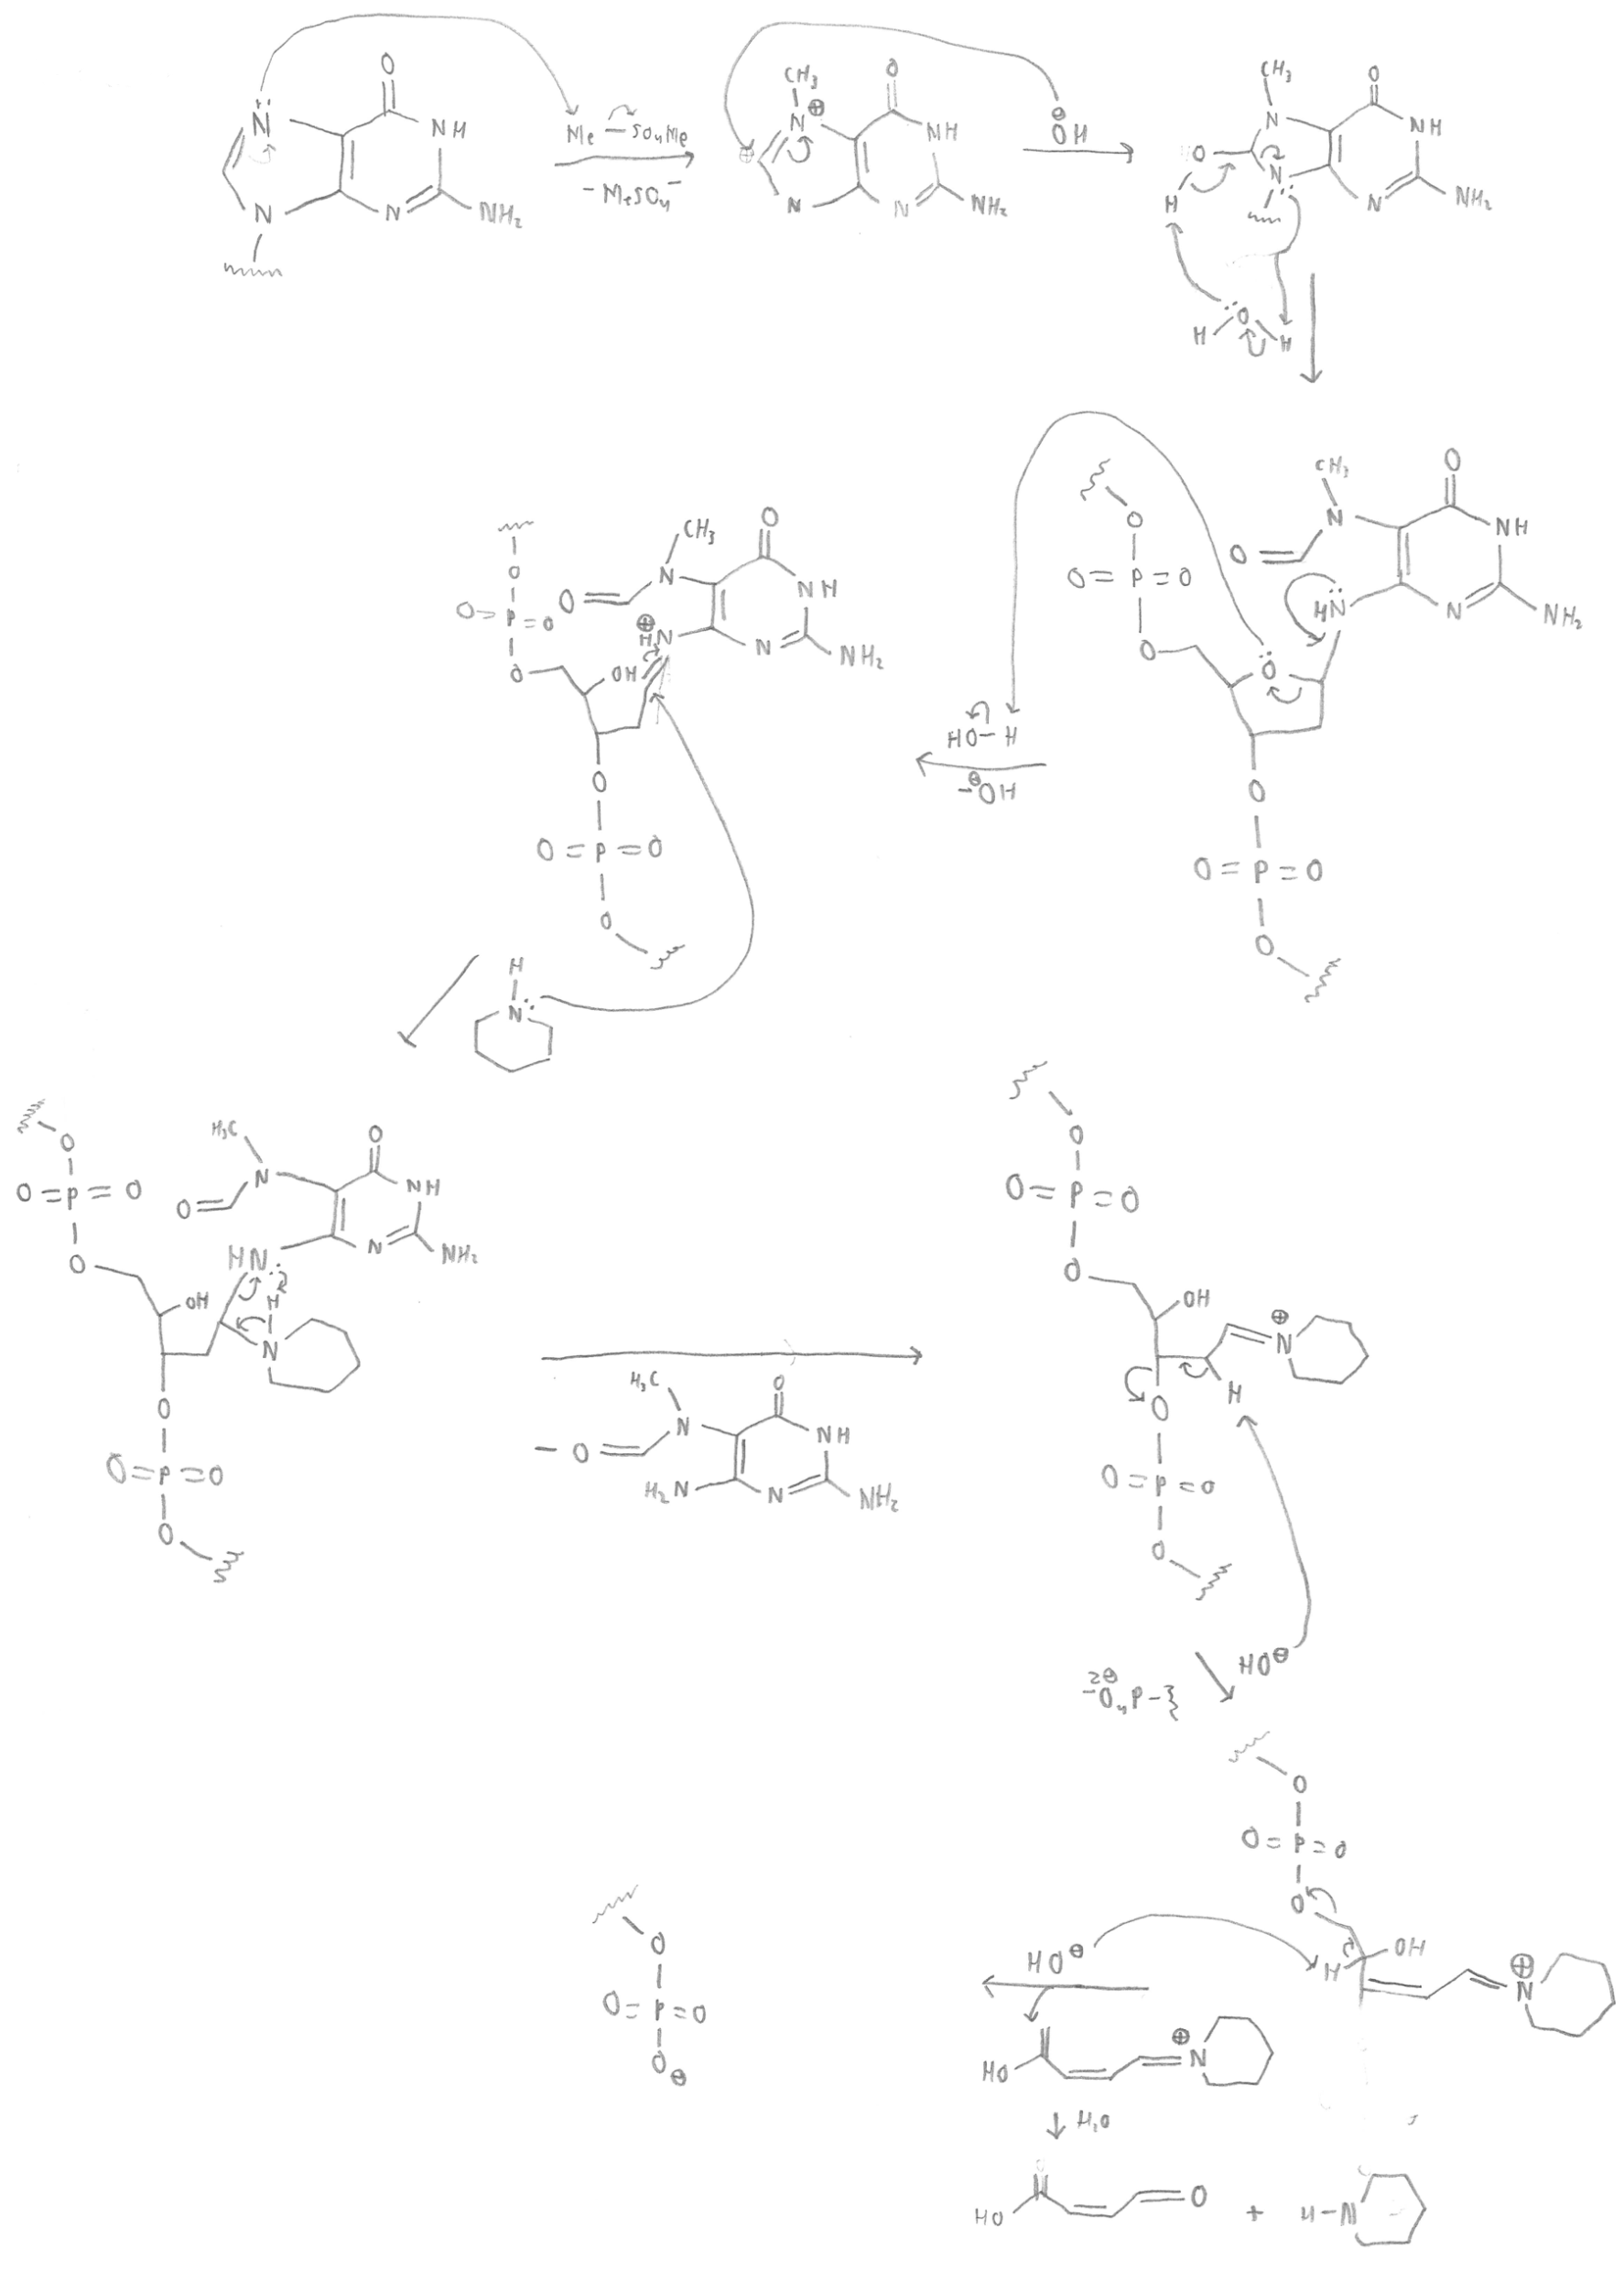
\includegraphics[width=\linewidth]{../ExtFiles/pset3-mechanismG.png}
                \caption{G.}
                \label{fig:pset3-mechanismG}
            \end{subfigure}
        \end{figure}
        \begin{figure}[H]
            \ContinuedFloat
            \centering
            \begin{subfigure}[b]{\linewidth}
                \centering
                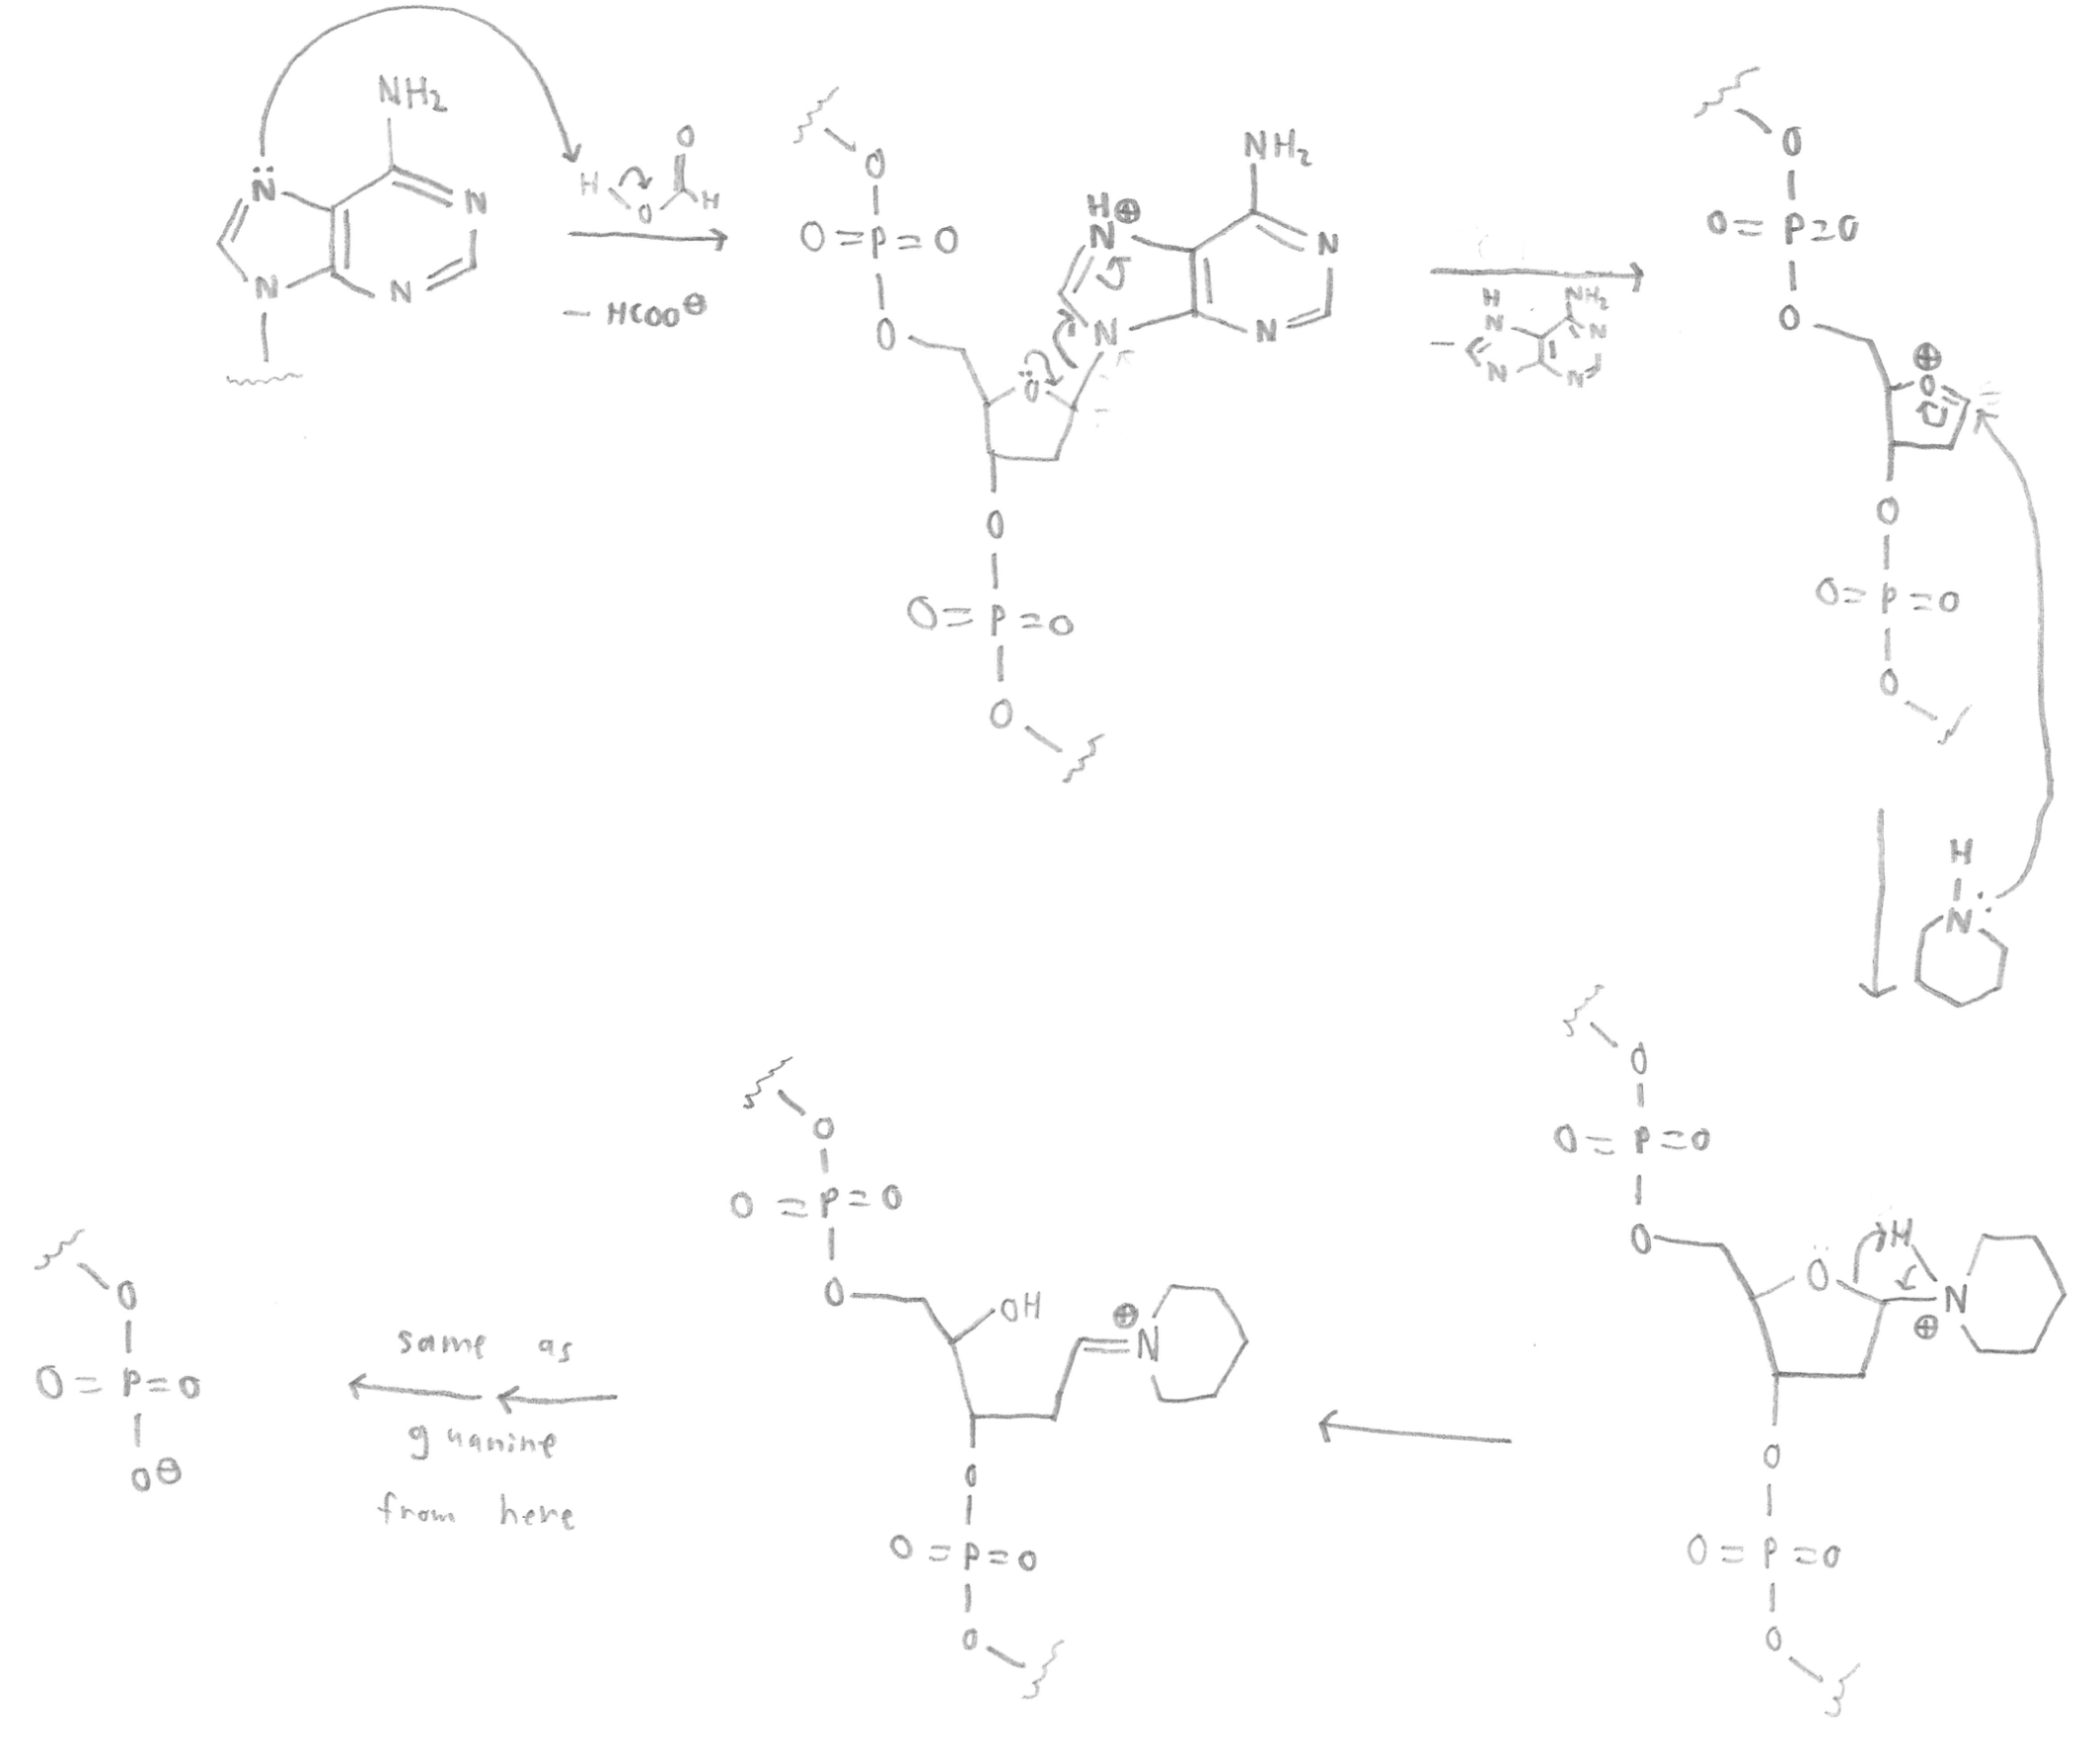
\includegraphics[width=\linewidth]{../ExtFiles/pset3-mechanismA.png}
                \caption{A.}
                \label{fig:pset3-mechanismA}
            \end{subfigure}
        \end{figure}
        \begin{figure}[H]
            \ContinuedFloat
            \centering
            \begin{subfigure}[b]{\linewidth}
                \centering
                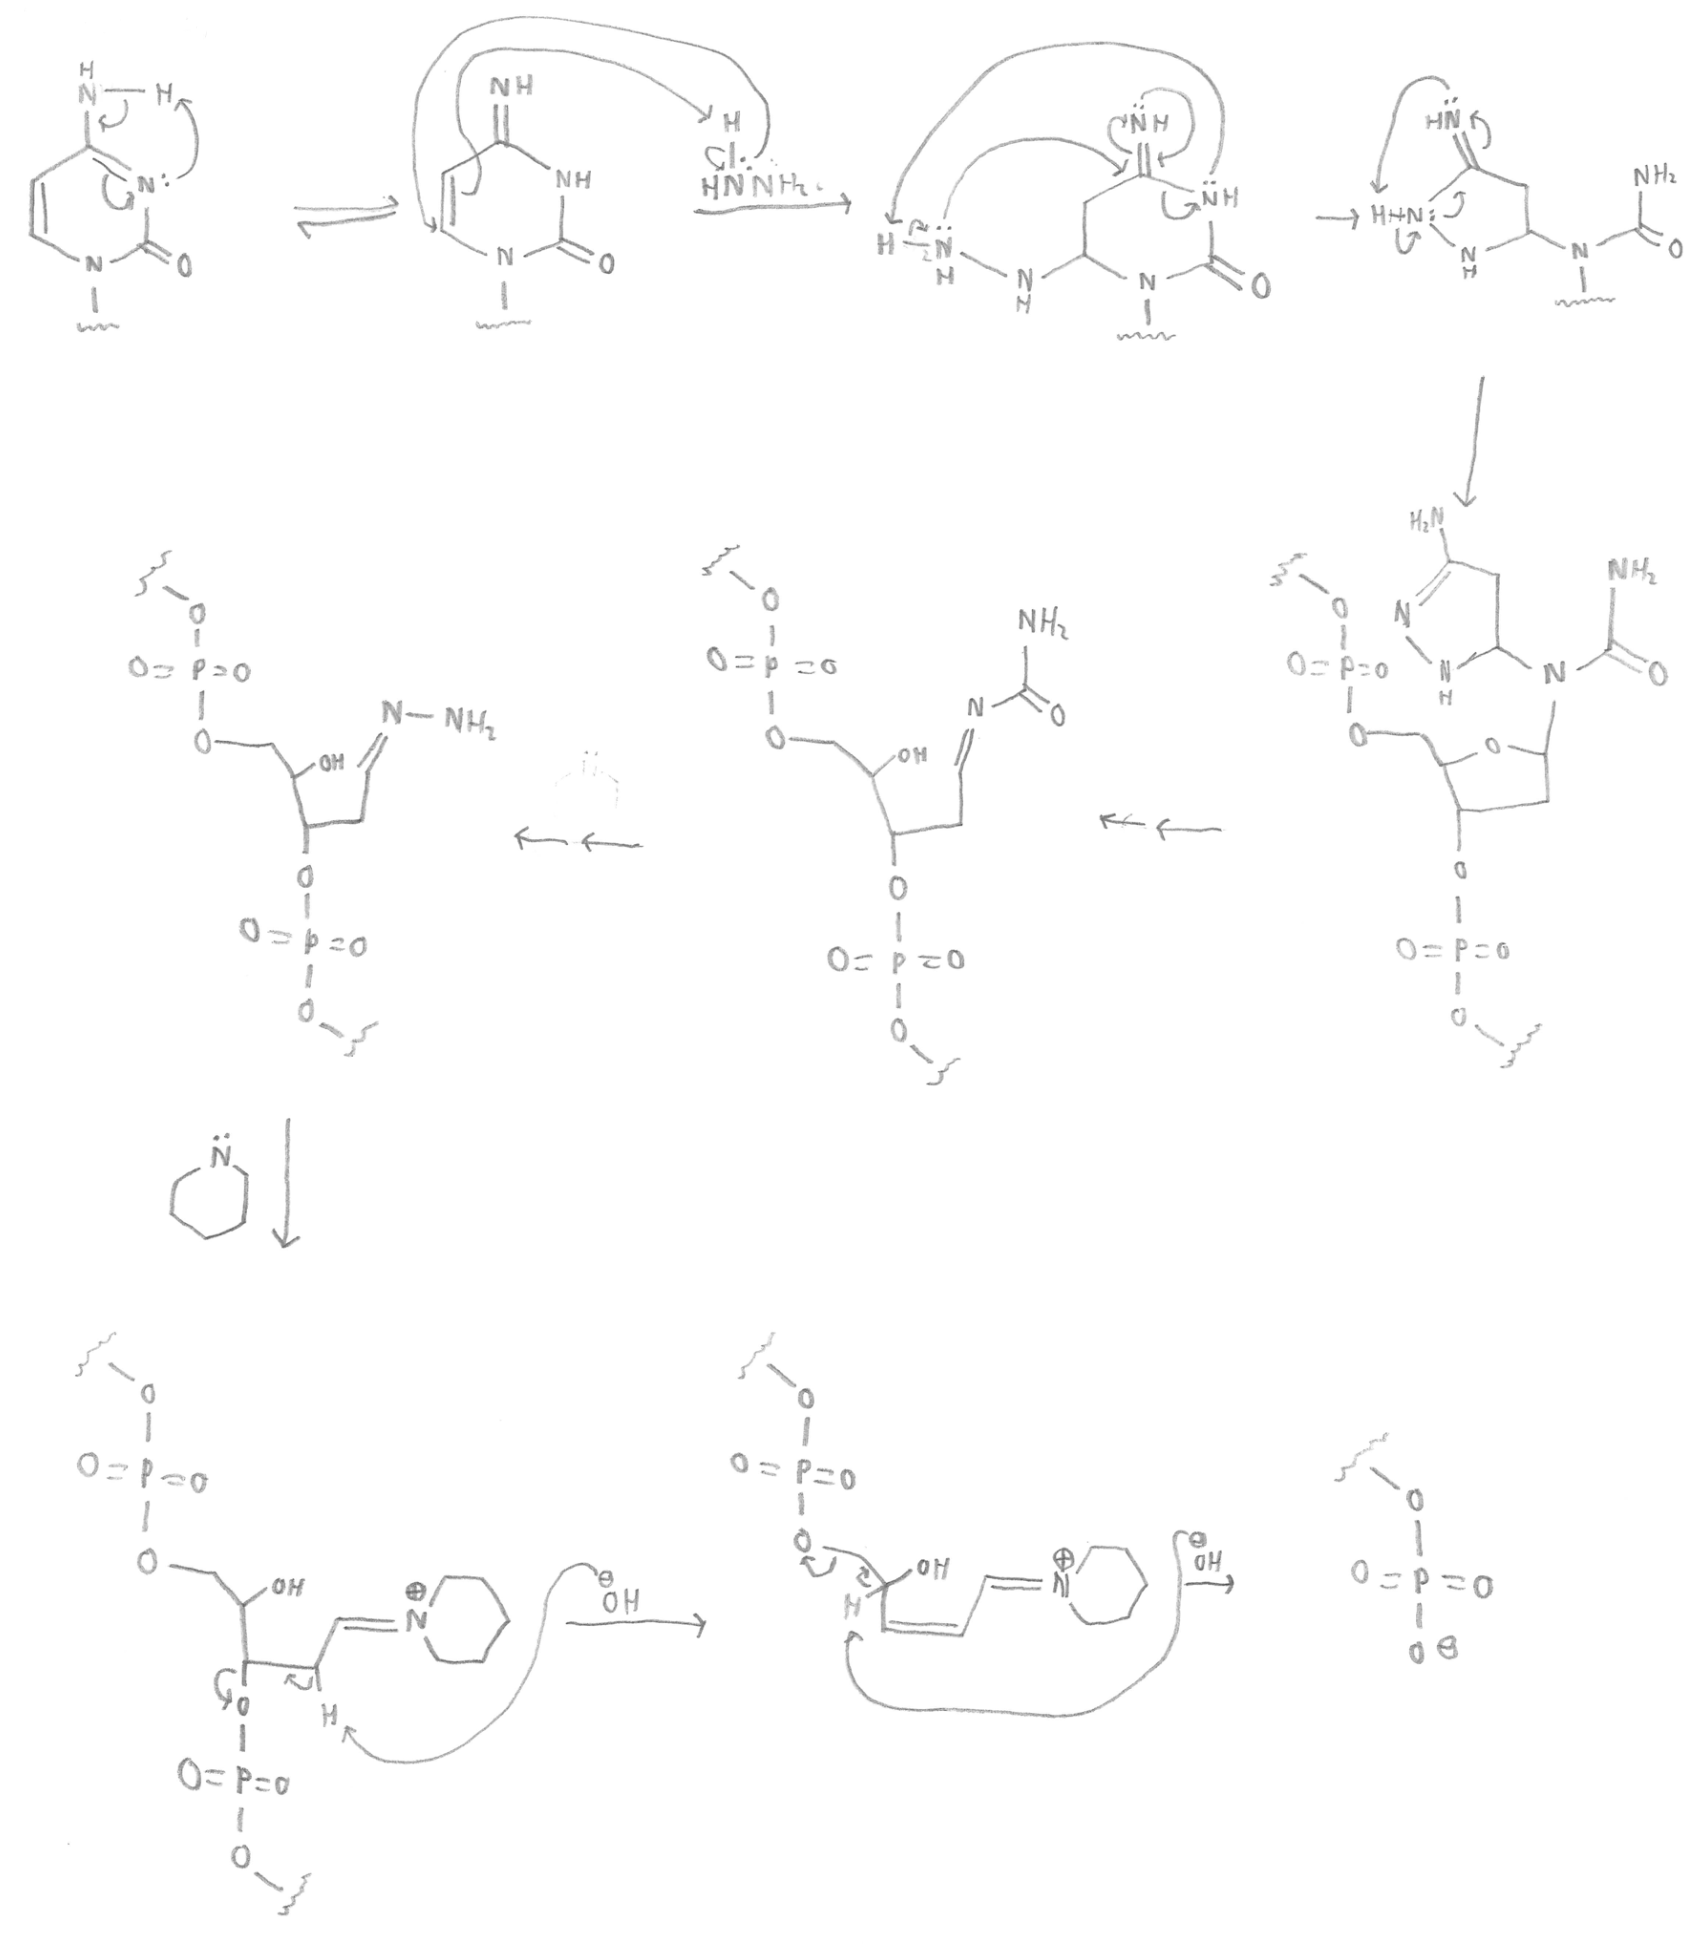
\includegraphics[width=\linewidth]{../ExtFiles/pset3-mechanismC.png}
                \caption{C.}
                \label{fig:pset3-mechanismC}
            \end{subfigure}
        \end{figure}
        \begin{figure}[H]
            \ContinuedFloat
            \centering
            \begin{subfigure}[b]{\linewidth}
                \centering
                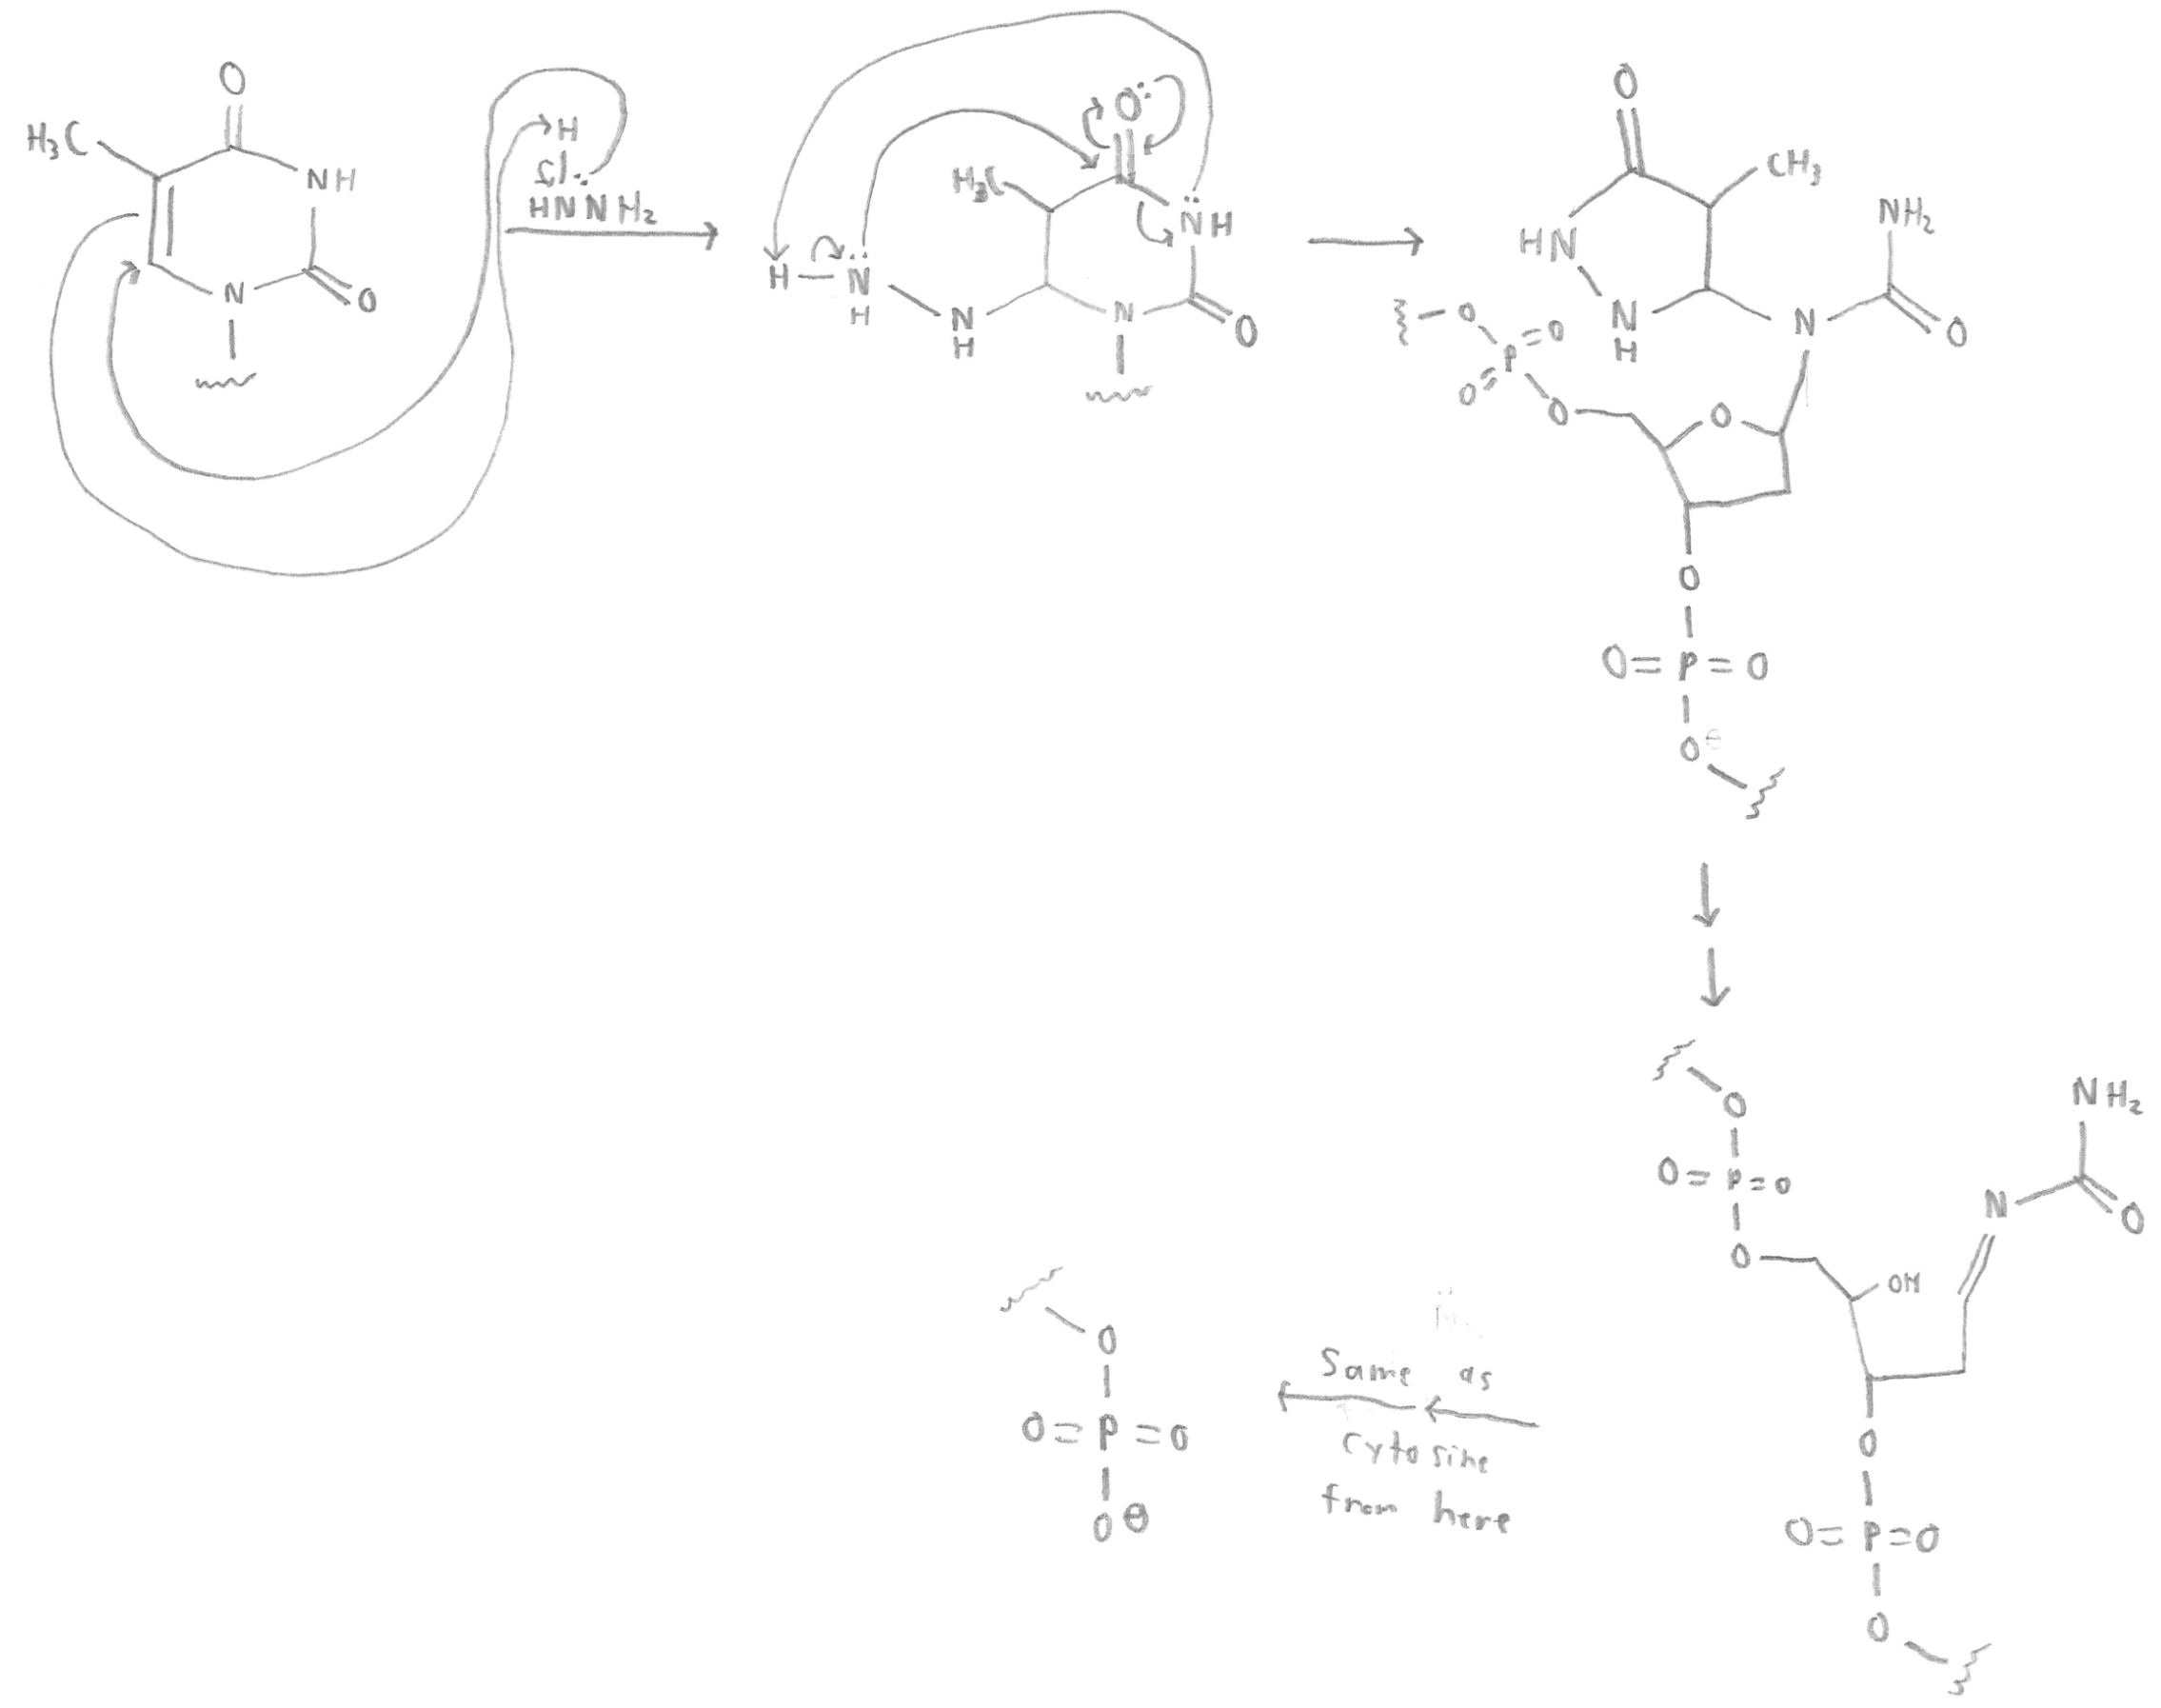
\includegraphics[width=\linewidth]{../ExtFiles/pset3-mechanismT.png}
                \caption{T.}
                \label{fig:pset3-mechanismT}
            \end{subfigure}
            \caption{Mechanisms.}
            \label{fig:pset3-mechanism}
        \end{figure}
        \vspace{-1em}
    \end{proof}
    \item Sequencing primer.\par
    Assuming the sequence of the human genome is completely random (it is not!), what is the minimum length of DNA primer you would need for it to bind only to a single site in the human genome? The number alone is invalid, unless accompanied by a calculation. (4 pts)
    \begin{proof}[Answer]
        The human genome contains \num{3e9} base pairs.\par
        A completely \emph{random} genome means that every sequence has an equal probability of occurring. Thus, for example, the 3 base pair sequence TGA has a $1/4^3$ chance of occurring (4 possible base pairs in each slot). Therefore, TGA will be present $\num{3e9}\cdot 4^{-3}$ times in the theoretical random human genome.\par
        We want to find the smallest $n$ such that a sequence of length $n$ occurs at most once. Thus, mathematically, we want to find the smallest $n\in\mathbb{N}$ such that
        \begin{equation*}
            \num{3e9}\cdot\frac{1}{4^n} \leq 1
            \quad\Longleftrightarrow\quad
            \log_4(\num{3e9}) \approx 15.74 \leq n
        \end{equation*}
        Therefore,
        \begin{equation*}
            \boxed{n = 16}
        \end{equation*}
    \end{proof}
    \item Plasma membrane and cell structure.
    \begin{enumerate}
        \item When a lipid bilayer snaps or breaks, why can it not repair itself by forming a hemi-micelle cap as shown in the figure below? (4 pts)
        \begin{figure}[h!]
            \centering
            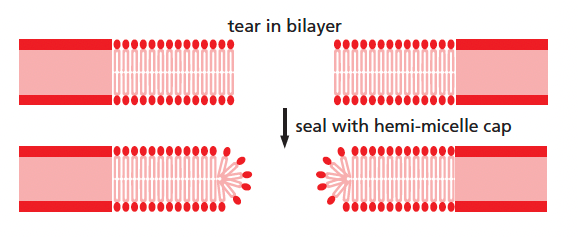
\includegraphics[width=0.4\linewidth]{../ExtFiles/pset3-hemiMicelle.png}
            \caption{Hypothetical hemi-micelle membrane repair.}
            \label{fig:pset3-hemiMicelle}
        \end{figure}
        \begin{proof}[Answer]
            % Packing of phospholipids is governed by their individual structures and, occasionally, protein binding. In general, a two-tailed phospholipid looks a lot like a cylinder leading to mostly flat packing, a phospholipid with more than two tails gives a conical shape and can cause the membrane to pucker inwards, and a phospholipid with a large glycolipid attached to its head group gives an inverted cone shape and can cause the membrane to pucker outwards. Additionally, a protein can bind multiple head groups and push them apart.\par
            % Protein-induced deformation is not relevant here because the plasma membrane is so thin that protein binding to a hypothetical hemi-micelle is unlikely. However, all the same, even a plethora of inverted cone-shape phospholipids is unlikely to be able to make a complete \ang{180} turn, let alone stay in the same place (the phospholipids actively move around and even flip between the sides of the plasma membrane).

            % Very few, if any, phospholipids would have large enough head groups to induce such bending, and there is no guarantee that they would stay in the same place, especially since the large head groups would probably want to get very far away from each other.


            Membrane puckering is induced by large head groups (e.g., glycolipids). Thus, to see such extreme bending, we would need a plethora of very large head groups in the very small area of the hemi-micelle. Energetically, this would be extremely unfavorable, and such groups would likely move away from each other very rapidly if ever brought so close together, returning the tear to its original form. Indeed, it will be far more energetically favorable for the two hydrophobic regions to just reunite into one continuous region.
        \end{proof}
        \item You are studying the binding of proteins to the cytoplasmic face of tumor associated macrophages for which you need a pure population of "inside-out vesicles" made from the plasma membrane. You have devised a method that gives a good yield of inside-out vesicles from the plasma membrane, but your preps are still contaminated with varying amounts of right-side-out vesicles. A senior grad student in the lab suggests that you pass your vesicles over an affinity column made of lectin coupled to solid beads. What is the rationale underlying her suggestion? (3 pts)
        \begin{proof}[Answer]
            If the population of vesicles is made from the plasma membrane of tumor associated macrophages, then any vesicles with right-side-out proteins will likely have sugars that can bind to lectin among them. Thus, when we pass the vesicles through an affinity column made of lectin coupled to solid beads, the lectin beads bind all right-side-out vesicles. All inside-out vesicles will pass through and not get stuck. Thus, such an affinity column is a valid method of purification.
        \end{proof}
    \end{enumerate}
    \item Protein export and import.\par
    Describe a strategy to position a fluorescent protein, say GFP, anchored to the inner mitochondrial membrane, but projecting into the intra-lumenal space. What are the steps that lie between the mRNA of this protein being translated, up until the protein is positioned as above? (7 pts)
    \begin{proof}[Answer]
        Herein, I will describe the strategy that makes use of the mitochondrial OXA complex.\par
        We assume that GFP already contains the correct primary and secondary localization/signal sequences (likely a translocation sequence on the C-terminus). If it does not, we should be able to add it either pre-translationally (by modifying the GFP-encoding mRNA) or post-translationally (a nuclear localization sequence can be fused with GFP per Lecture 6.1, so a mitochondrial localization sequence should be able to be attached, too). We also assume that the protein has made its way into the cytosol and can navigate (or be directed) to the mitochondrial outer membrane.\par
        Upon arrival at the mitochondria, the primary GFP localization sequence attaches to the receptor protein of the TOM complex and begins to be unwound and pulled in toward the intra-lumenal space. Since we are supposing an OXA pathway is used, the TOM and TIM complexes lock together, allowing translocation to happen all at once from the cytosol to the mitochondrial matrix. Successive ATP physphorylations of the complexes pull the protein through a few peptides at a time. Once the translocation sequence enters the matrix, a signal peptidase cleaves it off, exposing the secondary localization sequence. Once GFP is completely inside the matrix, TOM and TIM separate.\par
        Now inside the matrix, the secondary signal sequence sends GFP to the OXA complex. The OXA complex flips the protein so that the tag is in the inner membrane and the bulk of the protein is in the intra-lumenal space.
    \end{proof}
\end{enumerate}




\end{document}